%% 
\chapter{Information Content Analysis} \label{ch:info}

\section{Introduction}

The AERONET collects not only the multi-spectral and multi-angular radiance
observations, but also the state of light polarization from various viewing
angles over many sites (section \ref{subsec:cimel318}). 
Unfortunately, the potential of AERONET polarization
measurements in retrieving aerosol microphysical parameters has not been fully
exploited. Polarization measurements contain valuable information about aerosol
microphysical properties \citep{Mishchenko97,Cairns97}, as
the polarization of light is highly sensitive to the aerosol size and
refractive index \citep{Hansen74}. Several studies have emphasized the
usefulness of the polarimetric observations taken by the ground-based
instruments \citep{Cairns97, Boesche06, Emde10, Zeng08}.  
\citet{Vermeulen00} presented a two-step method to retrieve
aerosol microphysical properties from polarized radiances: first, the single
scattering albedo and the natural and polarized phase functions were retrieved
from transmission and almucantar radiances and polarization in the principal
plane; second, the aerosol PSD and refractive index were then derived. With the
current AERONET inversion algorithm, \citet{Dubovik06} conducted a case
study using polarization data in a UAE$^2$ (Unified Aerosol Experiment-United 
Arab Emirates) field campaign \citep{Reid08}. \citet{Li09} extended the
inversion algorithm of \citet{Dubovik06} to include multi-spectral
polarization and demonstrated improved retrievals in real part aerosol
refractive index for fine particles and the fraction of spherical particles.

However, questions regarding the use of AERONET polarimetric observations for
retrieving aerosol microphysical parameters remain unresolved: (1) Practically,
do the existing AERONET photo-polarimetric measurements have any potential to
improve the retrieval of aerosol information content that we now routinely
obtain from radiance measurement only? and (2) Hypothetically, how can future
upgrades of AERONET photo-polarimetric measurements and inversion algorithm
maximize the retrieval information content of aerosols? Answering these two
questions is not only relevant to the future AERONET instrumentation design,
but also for the ground-based passive polarimetric remote sensing of aerosols
in general. 

%% Table of a priori
\begin{table}[b]
  \centering
  \small
  \caption{The aerosol parameters defined for both fine and coarse aerosol
modes\textsuperscript{a}.}
  \label{tab:infox}
  \begin{tabular}{p{2em} C{3em}  C{3em} C{9em} C{9em} C{7em} }
  \toprule
  Mode  & $\reff$($\mu$m) & $\veff$ & $\mathbf{m}_\text{r}$ &
$\mathbf{m}_\text{i}$ & $\assa$ \\
  \midrule
  Fine & 0.21 \newline (80\%) & .25 \newline (80\%) &
    1.44, 1.44, 1.43, 1.42 \newline (.15) &
    .009, .011, .012, .011 \newline (.01) &
    .95, .93, .92, .91 \\
  Coarse & 1.90 \newline (80\%) & .41 \newline (80\%) &
    1.56, 1.55, 1.54, 1.54 \newline (.15) &
    .004, .003, .003, .002 \newline (.005) &
    .84, .91, .93, .96 \\
  \bottomrule
  \multicolumn{6}{m{35em}}{\textsuperscript{a}The complex refractive index
$\mathbf{m}_\text{r}-\mathbf{m}_\text{i}i$, and single scattering albedo
$\assa$ are reported at 440, 675, 870, and 1020 nm. Bracketed values are
assumed a priori error in relative for $\reff$ and $\veff$ and in absolute
for $\mathbf{m}_\text{r}$, $\mathbf{m}_\text{i}$, and $\assa$. }
  \end{tabular}
\end{table}

In this chapter, we seek to answer above questions from a theoretical 
perspective (section \ref{subsec:infotheory}) by investigating the available 
information contained in the AERONET measurements with and without the 
inclusion of polarization data. This investigation is to
provide the a theoretical foundation to support actual
algorithm development for using polarimetric data for aerosol retrievals. 
The structure of this chapter is as follows. In section \ref{sec:expdesign}, 
we describe the experimental design on the aerosol models, error 
characteristics of \textit{a priori} and AERONET measurements. Section
\ref{sec:inforesult} presents the results of information content and error
analysis. In section \ref{sec:infosensi}, we investigate the sensitivity of
retrieval uncertainties in aerosol parameters with respect to the aerosol
loading and fine/coarse aerosol characteristics. Finally, we summarize in
section \ref{sec:infosummary} the general findings of this study and 
implications for practical algorithm development. 

\section{Experimental Design} \label{sec:expdesign}

\subsection{\textit{a priori} characteritics}

The state vector $\xbf$ comprises 22 (11 pairs) retrieved parameters,
namely, the columnar volume concentration $V_0$, the effective radius $\reff$, the
effective variance $\veff$, and the complex refractive index $\mreal+\mimag{i}$ 
at 440, 675, 870, and 1020 nm (section \ref{subsec:xy}). These 11 pairs of 
parameters charcterizing aerosol properties in the both fine and coarse 
aerosol modes; each mode follows a lognormal PSD function. Table \ref{tab:infox} 
displays aerosol size parameters, refractive indices, and single scattering 
albedo for each size mode adopted for error and information analysis; 
also showed in brackets are their associated \textit{a priori} uncertainties. 
The fine-mode particles are corresponding to water-soluble aerosols 
obtained from OPAC database \citep{Hess98} with updates by \citet{Drury10}, 
while the coarse-mode is preassembly for large spherical particles with 
refractive index from \citet{Patterson77,Wagner12}.

%% Table of aerosol optical properties
\begin{table}[b]
  \centering
  \small
  \caption{The aerosol scenarios adapted for numerical
experiments\textsuperscript{a}.}
  \label{tab:infoopt}
  \begin{tabular}{p{8em} C{1em} C{1em} C{7em} C{7em} C{1em} C{7em} }
  \toprule
  Aerosol type & $V_0$ & $\fmfv$ & $\taua$ &
$\fmftau$ & AE & $\assa$ \\
  \midrule
  Fine-dominated & .15 & .8 & 1.0, .58, .36, .25 &
    .97, .95, .92, .88 & 1.5 & .95, .93, .92, .91 \\
  Well-mixed & .22 & .5 & 1.0, .61, .41, .32 &
    .90, .83, .74, .65 & 1.3 & .94, .93, .92, .93 \\
  Coarse-dominated &.43 &.2 & 1.0, .71, .57, .50 &
    .69, .55, .42, .32 & .82 & .91, .92, .92, .94 \\
  \bottomrule
  \multicolumn{7}{m{35em}}{\textsuperscript{a}Values for $\taua$, $\assa$, and
$\fmftau$ are listed respectively for spectral wavelength of
440, 675, 870, and 1020 nm. The AE is reported between 440 and 870 nm. $V_0$ is 
in the unit of $\mu$m$^3\mu$m$^{-2}$}
  \end{tabular}
\end{table}

In order to include various atmospheric conditions, we simulate three types of
aerosols---each with different relative percentage between the coarse and fine
modes---(I) fine particles dominated, (II) well mixed, and (III) coarse
particles dominated. As listed in Table \ref{tab:infoopt} and illustrated 
in Figure \ref{fig:infopsd}, fine-mode
fractions in terms of volume ($\fmfv$) are defined as 0.8, 0.5, and 0.2 for these
three types, respectively. Aerosol volumes are scaled as necessary to maintain
a normalized AOD at 440 nm corresponding to a moderate hazy condition
($\tau_{440}=1.0$). The spectral aerosol optical depths $\taua$, 
single scattering albedo $\assa$, and the Ångström exponent (AE) 
are calculated and also shown in Table \ref{tab:infoopt}. 

\begin{figure}[t]
  \centering
  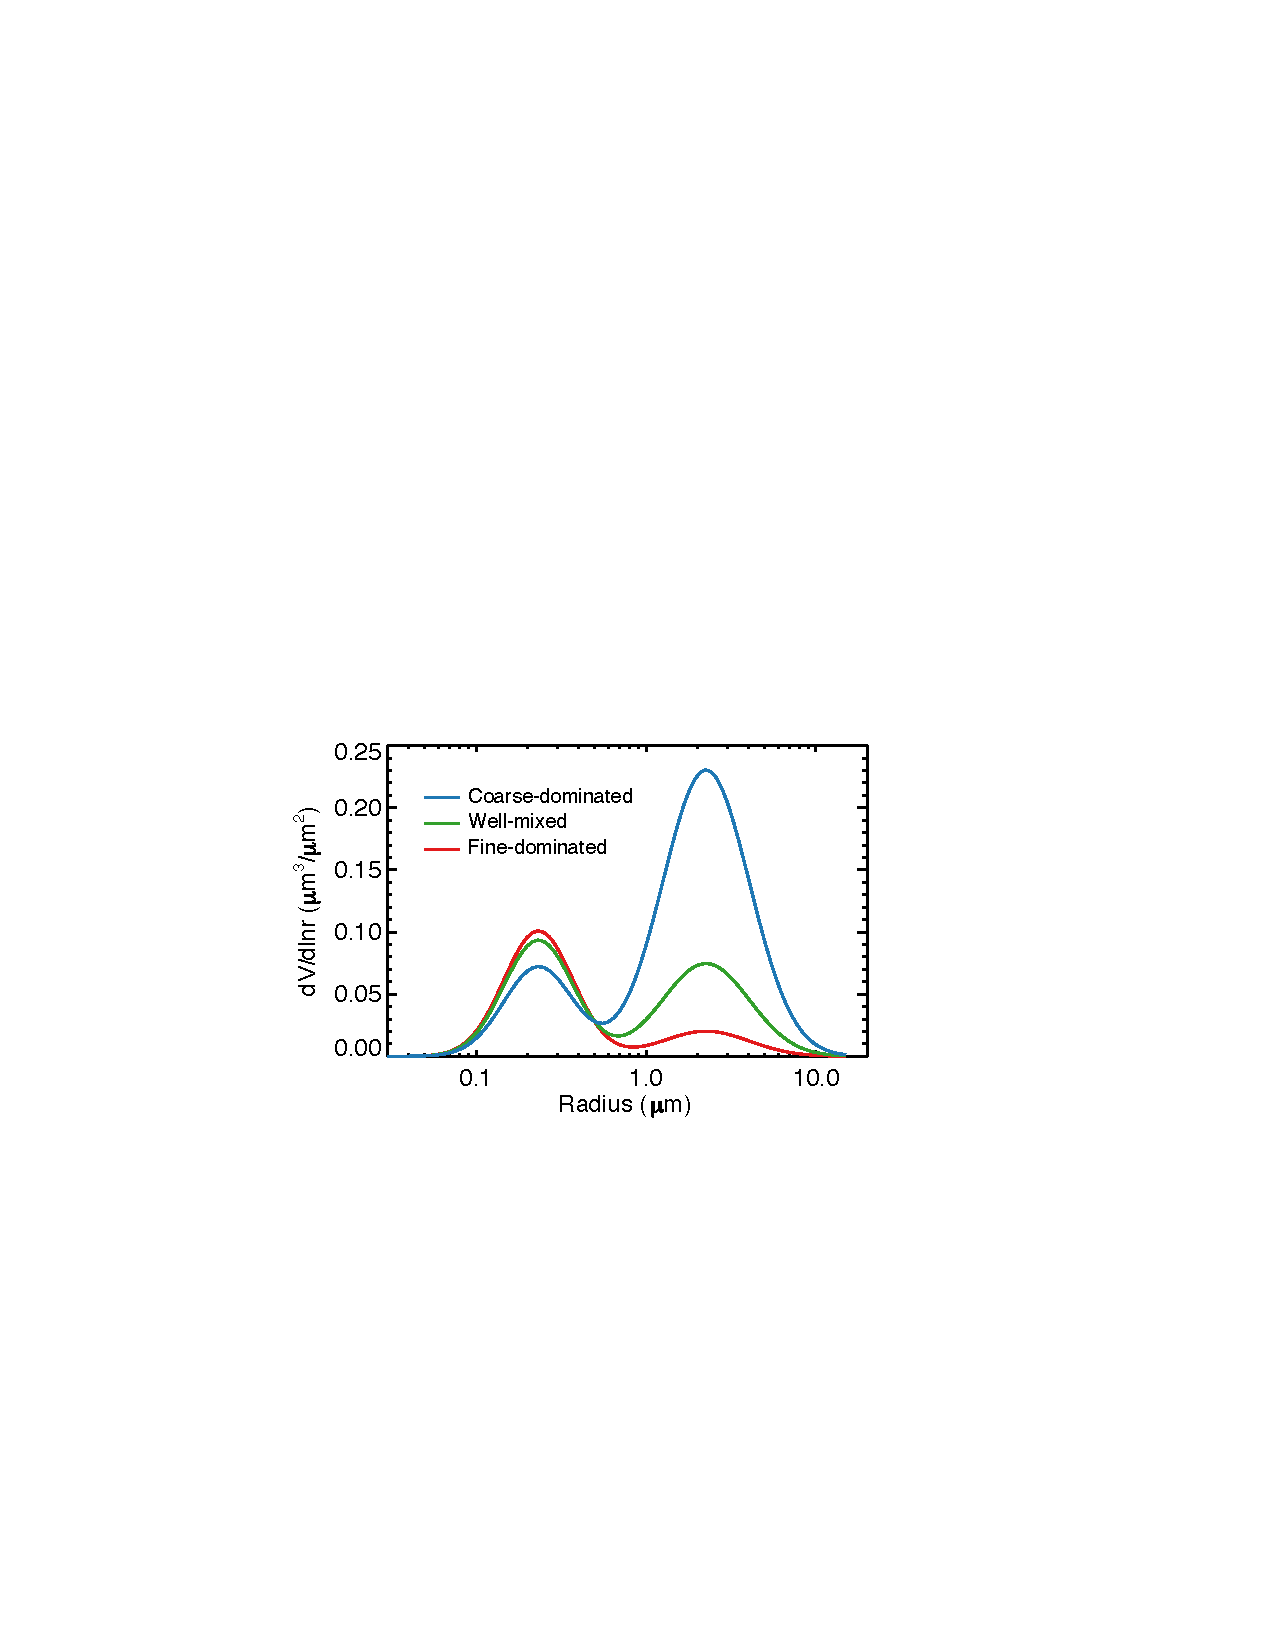
\includegraphics[width={0.75\textwidth}]{figures/info01.pdf}
  \caption{Volume size distribution for the aerosol types adopted for the
information analysis. Relevant aerosol parameters are summarized in the Tables
\ref{tab:infox} and \ref{tab:infoopt}.}
  \label{fig:infopsd}
\end{figure}

\subsection{Synthetic observations}

As described in section \ref{subsec:cimel318} and Table \ref{tab:cimel318}, 
The SunPhotometer equipped at AERONET sites routinely measures direct and
diffuse (sky) solar radiances and optionally the mono-band light 
polarization \citep{Holben98}. Recently, multi-spectral polarizations 
have also been taken with a newer-generation SunPhotometer (CIMEL CE318-DP) 
at some sites \citep{Li09} and the UAE$^2$ fields campaign \citet{Reid08}.
 Here we focus our study on using multi-spectral polarizations 
for the inversion of aerosol parameters. 

In order to investigate the merit of synergizing various observations in the
inversion, we define four different scenarios of observation vectors, i.e., I1,
I2, P1, and P2 as summarized in the Table 1. The observation vector in scenario
I1 comprises direct sun AODs and solar almucantar radiances ($\ialm$) at 440,
675, 870, and 1020 nm. Scenario I2 includes measurements in scenario A and the
total radiances ($\ipp$) at the same four wavelengths observed in the solar
principal-plane. Observations in scenario P1 are defined to further include
$\dolppp$ at those four wavelengths. Lastly, scenario P2 observations comprise
basic measurements in scenario I1 plus almucantar polarization ($\dolpalm$) at
same wavelengths. The $\dolpalm$ is not routinely measured by any current
SunPhotometer, but we include it for a comparative analysis. Measurements
defined in scenario I1 represent observations used by the current AERONET
operational inversion and thus serves as a control experiment. From scenario
I2, we can investigate the synergy of radiances in both the solar almucantar
and solar principal-plane. Scans in the solar principal-plane can achieve
larger scattering angles and thus may contain additional scattering
information. And with scenarios P1 and P2 we will be able to evaluate the
potential of adding polarization in the inversion. 

%% Table of aerosol optical properties
\begin{table}[t]
  \centering
  \small
  \caption{List of scenarios of AERONET observations used for
information content analysis.}
  \label{tab:infoy}
  \begin{tabular}{p{4em} p{11em} p{21em} }
  \toprule
  Scenario & Observations included\textsuperscript{a} & Remark  \\
  \midrule
  I1 & $\taua$, and $\ialm$ & Observations used in \Dub algorithm \\
  I2 & $\taua$, $\ialm$, and $\ipp$ & Scenario I1 plus principal-plane
radiances \\
  P1 & $\taua$, $\ialm$, $\ipp$ and $\dolppp$ & Scenario I2 plus
principal-plane polarization\\
  P2 & $\taua$, $\ialm$, and $\dolpalm$ & Scenario I1 plus almucantar
polarization \\
  \bottomrule
  \multicolumn{3}{m{35em}}{\textsuperscript{a}Variables are for four spectral
wavelengths, i.e., 440, 675, 870, and 1020 nm.}
  \end{tabular}
\end{table}

We exclude $\ippl$ (Table \ref{tab:cimel318}) in our analysis because 
sky radiance in the solar principal plane can be also obtained during the 
polarization scan ($\ipp$). $\ippl$ and $\ipp$
are different in the viewing-angle sequences, but they generally share a
similar range of scattering angles. Thus, one is redundant for the other. We
also exclude analysis for monochromatic polarization (at 870 nm) current
measured on many AERONET sites, because single-band polarization measurements
contain much less information than multi-band ones and newer generation
SunPhotometers with multi-band polarization capacity will be deployed at more
AERONET sites. 

\section{Results} \label{sec:inforesult}

Following the approach stated in section \ref{sec:invtheory}, 
we have simulated the AERONET photo-polarimetric measurements under various 
solar zenith angles from 40$^\circ$ to 75$^\circ$ for the three 
defined aerosol types (Table \ref{tab:infoopt}). The simulated radiances 
($\ialm$) on the solar almucantar plane and the degree of linear 
polarization ($\dolppp$) on the solar principal plane are illustrated in 
Figure \ref{fig:infosimu} for aerosols of type II with solar zenith angle of 
55$^\circ$. These simulations for other aerosol types and other
solar zenith angles are of similar pattern. According to Figure
\ref{fig:infosimu}a, $\ialm$ decreases as the scattering angle increases, 
resulting from forward-dominated scattering phase function of aerosol 
particles. The maximum $\dolppp$ takes place at the scattering angle of 
90$^\circ$ as a result of composite effect of Rayleigh and aerosol scattering, 
while the smaller $\dolppp$ values dominates at the small scattering angles 
because of the predominance of diffracted light (Figure \ref{fig:infosimu}b).
With the synthetic data and relevant error characterizations, we have computed
the EN Jacobian matrix, DFS, and a posteriori error to evaluate the capacity of
AERONET measurements in inferring aerosol microphysical properties. Our
analysis mainly focuses on the comparison of those quantities between
measurements with and without including polarization, so that we can understand
the importance of adding polarization for the retrieval.  

\begin{figure}[t]
  \centering
  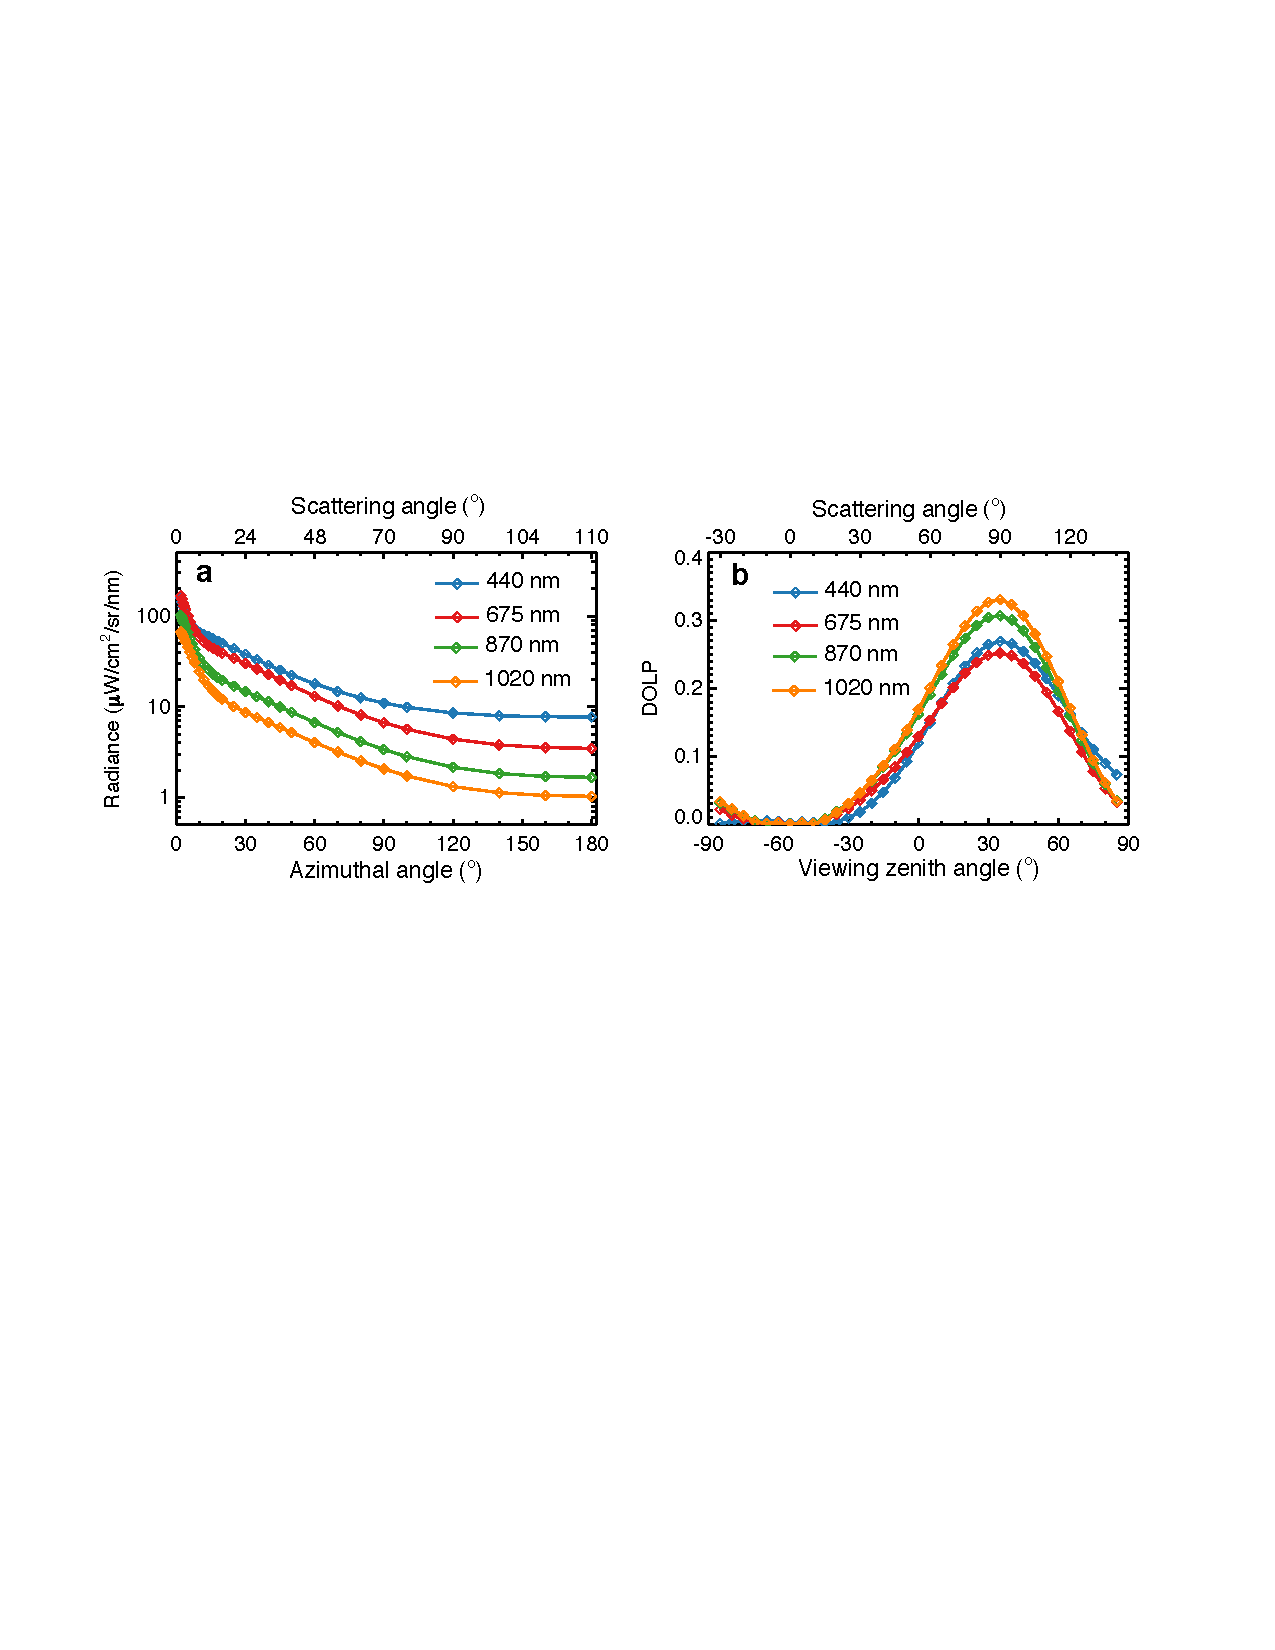
\includegraphics[width={\textwidth}]{figures/info02.pdf}
  \caption{(a) Simulated radiances in the solar almucantar plane as a function
of azimuth angle. (b) Simulated degree of linear polarization (DOLP) in the
solar principal plane as a function of view zenith angle. Simulations are for
the well-mixed aerosol type with columnar AOD of 1.0 at 440 nm as shown in the
Table \ref{tab:infoopt}. Solar zenith angle is 55$^\circ$ and top abscissas 
show corresponding scattering angles.}
  \label{fig:infosimu}
\end{figure}

\subsection{Error-normalized (EN) Jacobian matrix} \label{subsec:enj}

We compare the EN Jacobians for the $\ialm$ and $\dolppp$ in both 
Figure \ref{fig:infoenjf} and Figure \ref{fig:infoenjc} to disclose the 
importance of $\dolppp$ measurements to the retrieval. Distinct patterns of EN 
Jacobians can be found between the $\dolppp$ and $\ialm$ over the
scattering angle. As shown in Figures \ref{fig:infoenjf}a and
\ref{fig:infoenjc}a, the radiance at scattering angles less than
$\sim$10$^\circ$ decreases with increasing fine-mode aerosol loading (e.g.
negative $\partial\ialm/\partial{V_0}$) and increases with increasing 
coarse-mode aerosol loading (e.g. positive $\partial\ialm/\partial{V_0}$), 
whereas the sensitivity of the $\ialm$ to $V_0$ at larger scattering angles is 
larger positive in the fine mode and less positive in the coarse mode. 
It is because large particles scatter more radiation than small particles at 
near-forward scattering angles \citep{vandeHulst81}. In contrast, the $\dolppp$ 
presents profound sensitivity to the $V_0$ of aerosol in both modes at the 
scattering angles between 45$^\circ$ and 135$^\circ$ (Figures 
\ref{fig:infoenjf}f and \ref{fig:infoenjc}f). 

%% Figure EN Jacobian fine mode
\begin{figure}[p]
  \centering
  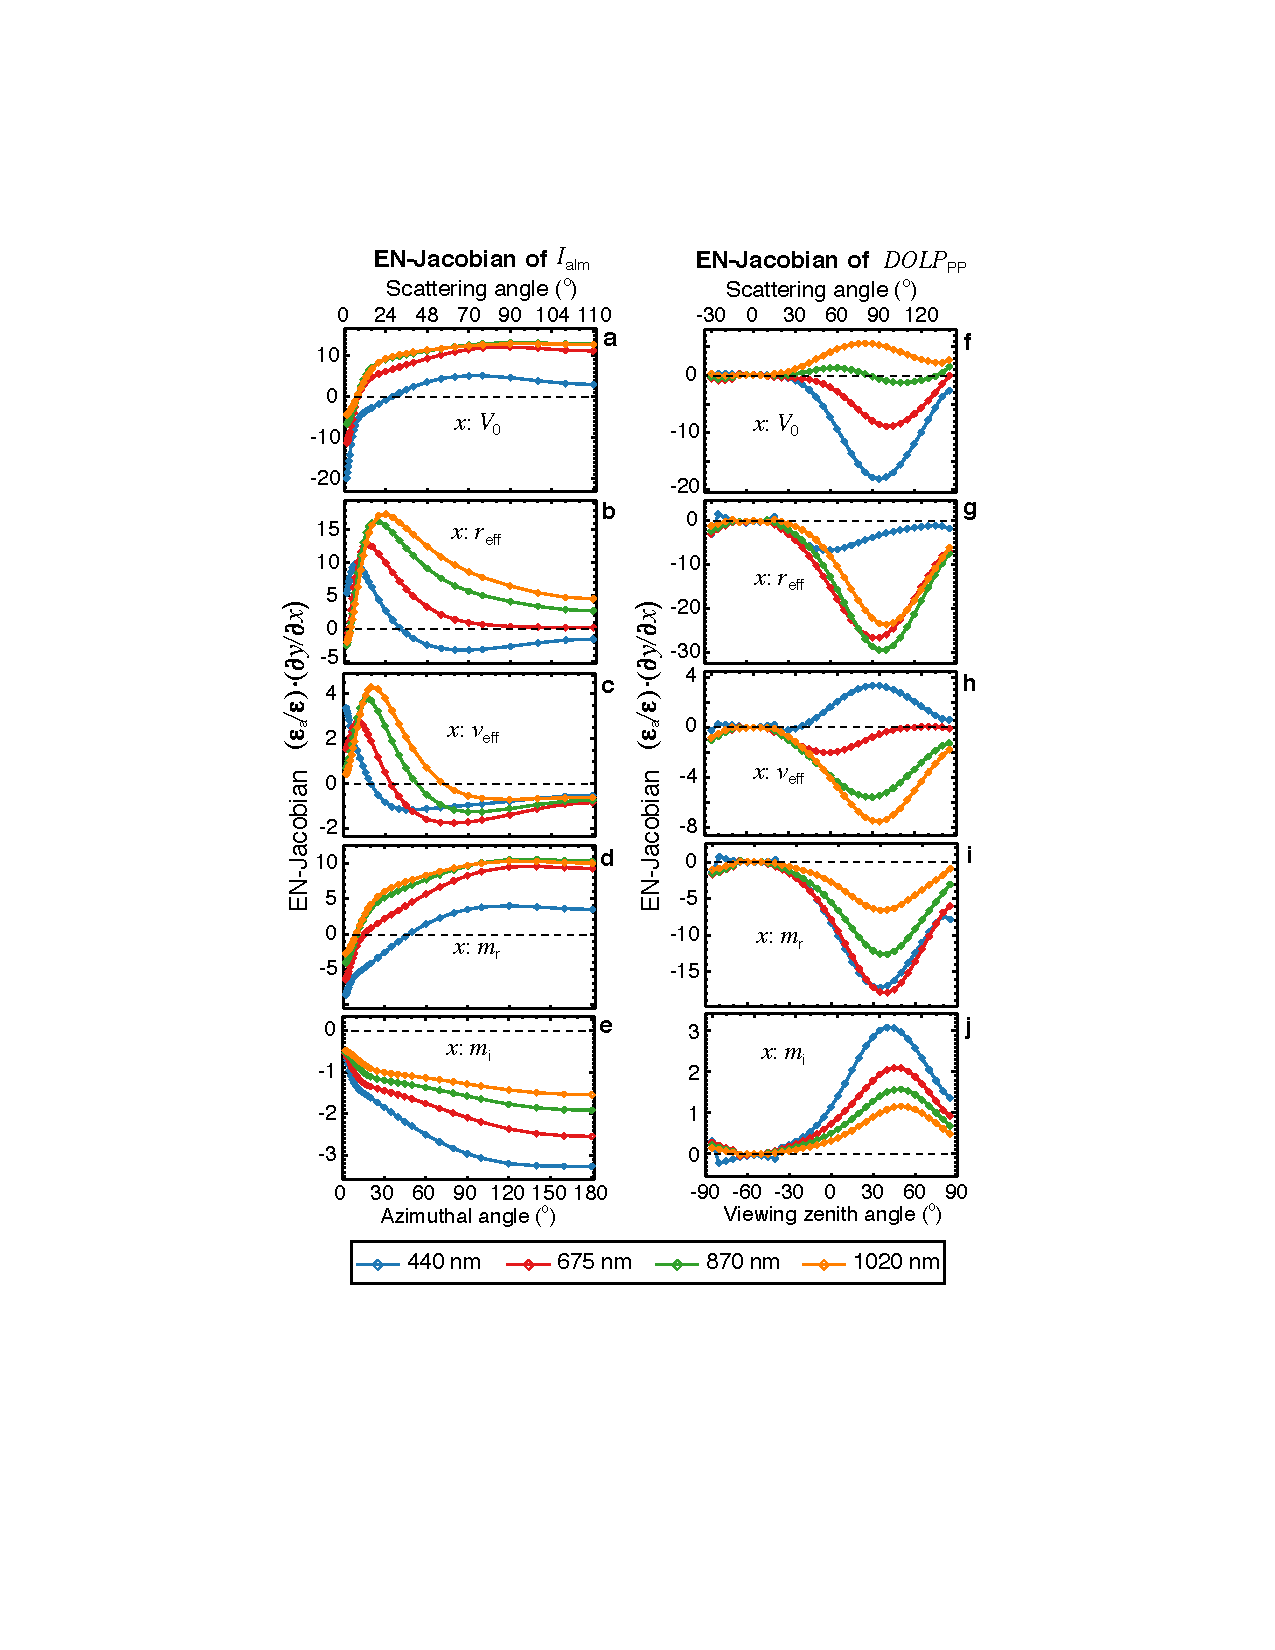
\includegraphics[width={0.8\textwidth}]{figures/info03.pdf}
  \caption{Error-normalized Jacobians of almucantar radiances $\ialm$ (left
column) and degree of linear polarization $\dolppp$ (right column) with respect
to retrieved aerosol parameters in the \textit{fine} mode: (a, f) $V_0$, (b, g)
$\reff$, (c, h) $\veff$, (d, i) $\mreal$, and (e, j) $\mimag$. Simulations use
type-II aerosols with columnar AOD of 1.0 at 440 nm and solar zenith angle of 
55$^\circ$. The top and bottom abscissas are respectively the scattering angle
and SunPhotometer scanning geometries.}
  \label{fig:infoenjf}
\end{figure}

%% Figure EN Jacobian Coarse mode
\begin{figure}[p]
  \centering
  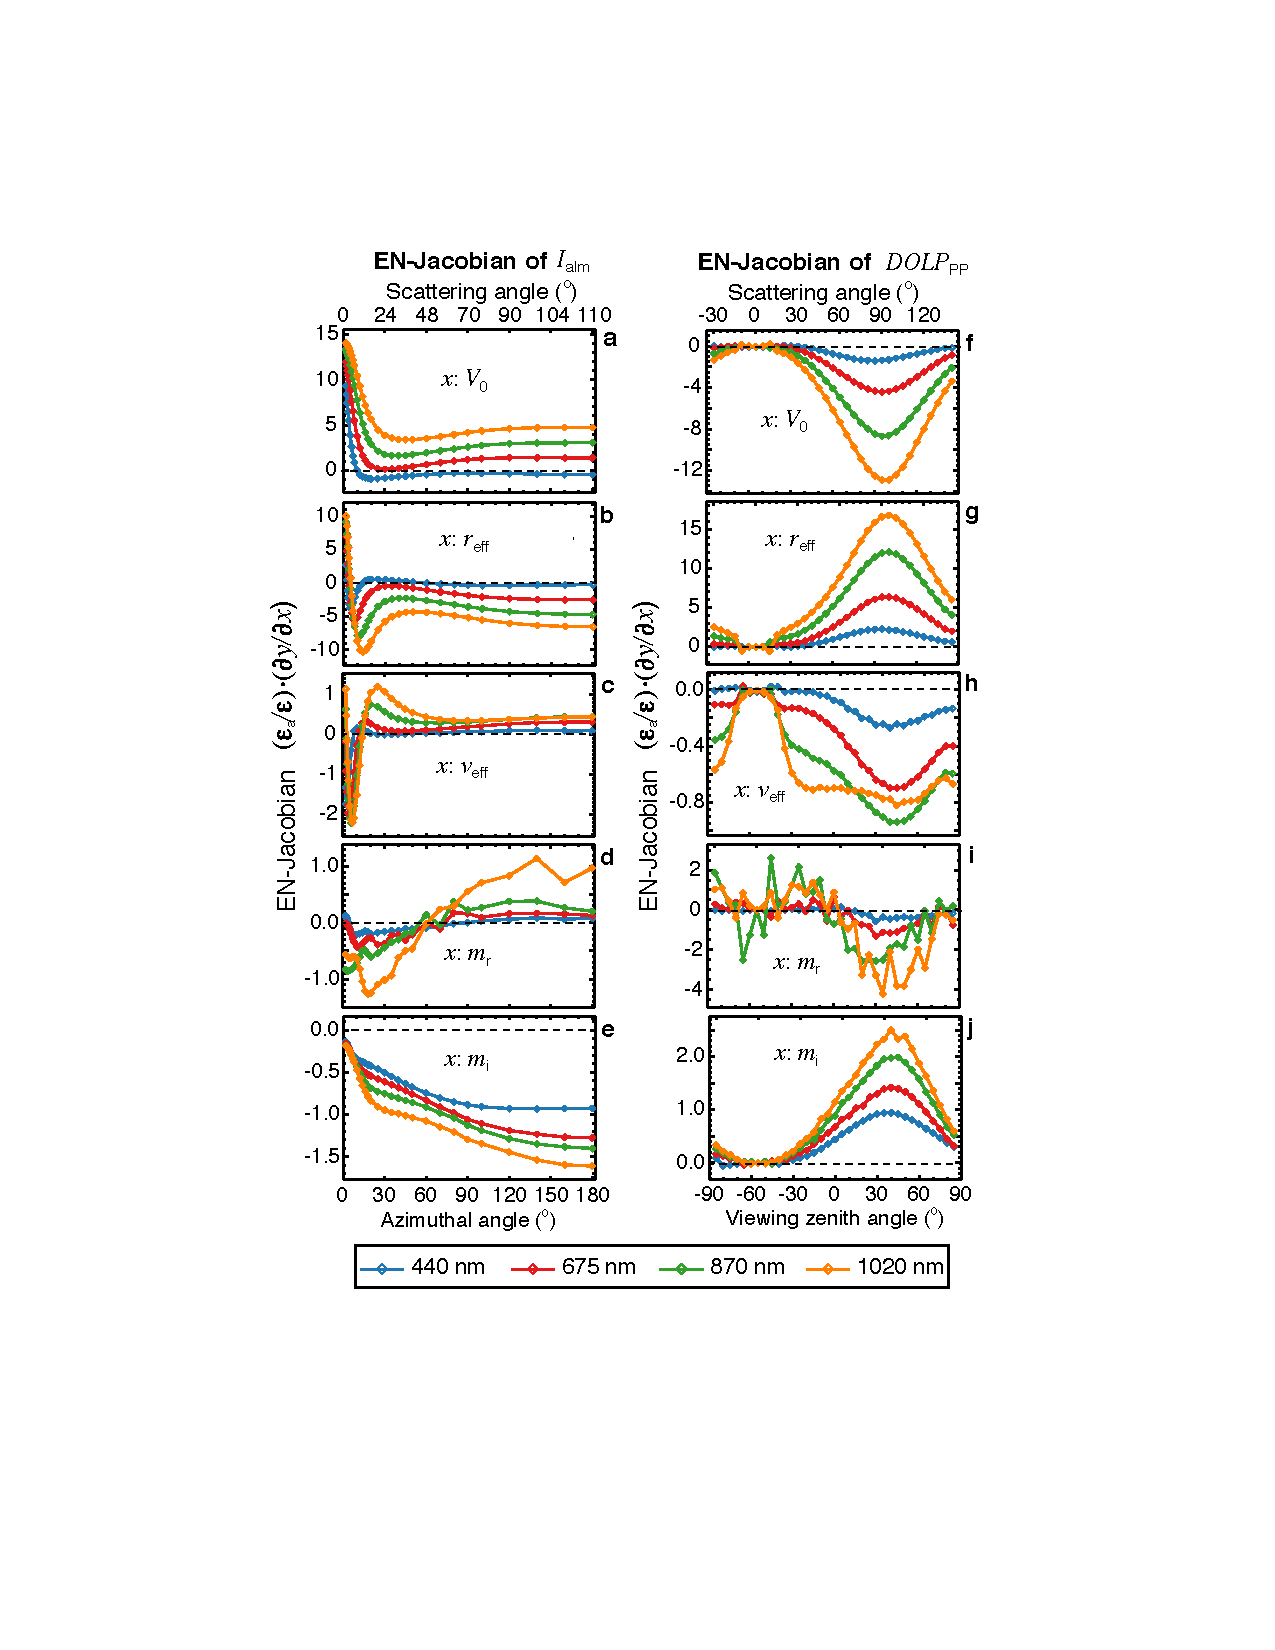
\includegraphics[width={0.8\textwidth}]{figures/info04.pdf}
  \caption{Same as Figure \ref{fig:infoenjf} but for parameters of aerosol in 
the \textit{coarse} mode.}
  \label{fig:infoenjc}
\end{figure}

Furthermore, the EN Jacobians of $\ialm$ and $\dolppp$ can also be synergized 
in terms of their variations on the spectral wavelength. For example, the EN
Jacobians for $\ialm$ with respect to the fine-mode $V_0$ express lowest at 
440 nm (blue curve in Figure \ref{fig:infoenjf}a), but those for $\dolppp$ at 
440 nm (blue curve in Figure \ref{fig:infoenjf}f) are largest ones among these
four spectral bands. Indeed, variations of these sensitivities with wavelength
are mainly determined by the change of size parameter $\eta$, which defined 
as the ratio of the particle size to the applied spectral wavelength, 
$\eta=2\pi\reff/\lambda$. The $\dolppp$ in scattering angles near 90$^\circ$
approaches unity under pure Rayleigh scattering regime where $\eta \ll 1$. 
When the  $\eta$ increases, the value of $\partial\dolppp/\partial{V_0}$ 
decreases and transits into negative at $\eta \sim 2$, reaches negative 
maxima at $\eta \sim 10$, then increases and slowly transits back to positive
when $\eta$ is as large as $\sim 40$ \citep{Hansen74}. The magnitude of the 
$\eta$ at these four bands ranges from 3.0 to 1.3 for the fine-mode particles 
and from 27 to 11 for the coarse-mode particles. Therefore we can understand 
that: (i) the sensitivity of $\dolppp$ to the fine-mode $V_0$ is
positive at 1020 nm due to the small size parameter $\eta=1.3$ (orange curve 
in Figure \ref{fig:infoenjf}f); (ii) this sensitivity gets weaker at 675 nm to
 870 nm and transits to negative at 440 nm as $\eta$ increases 
(Figure \ref{fig:infoenjf}f); and (iii) this sensitivity for aerosol in the 
coarse mode is more negative for longer wavelengths that are
corresponding to smaller values of $\eta$. 

We also note that sensitivity of the $\ialm$ to PSD parameters dominates for
scattering angles less than $\sim$40$^\circ$ (Figures \ref{fig:infoenjf}b-c and 
\ref{fig:infoenjc}b-c), while its sensitivity to $\mreal$ and $\mimag$ 
prevails at larger scattering angles (Figures \ref{fig:infoenjf}d-e and
\ref{fig:infoenjc}d-e). In the near-forward scattering angular regions, the 
dominant scattering effect is the diffraction of light, which essentially 
depends on the size of particles and is independent of the index of refraction
\citep{vandeHulst81, Hansen74}. The $\dolppp$, in contrast, is sensitive to both
the aerosol size and the refractive index at scattering angles from 45$^\circ$ 
to 135$^\circ$ (right columns of the Figures \ref{fig:infoenjf} and
\ref{fig:infoenjc}). Variations of the sensitivity among spectral bands can be
explained by the wavelength-dependent size parameters as discussed in the above
paragraph.  

Overall, the $\dolppp$ EN Jacobians have similar or larger magnitudes to these of
$\ialm$, indicating that the $\dolppp$ measurements possess equal or larger
information for the inversion of these aerosol properties. Adding such
complementary $\dolppp$ measurements to the current radiance-only inversion can
potentially increase the retrieval accuracy. The magnitude of EN Jacobian
elements varies among retrieved parameters, which leads to the variability of
retrieval accuracy. The EN Jacobians with respect to the $V_0$ and $\reff$ of both
modes and the fine-mode $\veff$ and refractive index are larger than those of
other parameters. Correspondingly, these parameters are expected to achieve
higher accuracy in the retrieval. While the maxima in EN Jacobians of $\ialm$
with respect to the coarse-mode refractive index at 870 and 1020 nm slightly
excess unity (Figure \ref{fig:infoenjc}d-e), larger counterparts for $\dolppp$ 
(Figure \ref{fig:infoenjc}i-j) will likely result in improved retrievals. 
In contrast, magnitudes of EN Jacobian for both $\ialm$ and  $\dolppp$ with 
respect to coarse-mode refractive index at 440 and 675 nm are smaller than 
unity across the whole angular range. Adding polarization may not improve the
retrieval for coarse-mode refractive index at those shorter wavelengths in 
such aerosol scenario. However, the consideration of spectral dependence of 
refractive index by using the smoothness constraints will potentially resolve
this problem \citep{Dubovik04}.

\subsection{Information content and retrieval error}

We calculated the averaging kernel matrix $\Abf$, DFS, and \textit{a
posteriori} error for retrieved parameters from these four scenarios of 
observation defined in Table \ref{tab:infoy}. Figuress \ref{fig:infodfs1}a-c 
illustrate how the DFS varies with the solar zenith angles for
three defined aerosol types. The DFS in the scenario I2 (red curves) ranges
from 14 to 15 for the fine-dominated aerosol model, and from 17 to 19 for other
two aerosol models, about 2–3 degrees higher than those using AODs and $\ialm$
measurements in the scenario I1 (black curves), indicating that sky radiances
in the principal plane ($\ipp$) contain additional information. The scenario P1
(green curves), which comprises solar almucantar sky radiances and
principal-plane polarimetric radiances at four wavelengths, further increases
DFS by 1–2. Observations in the scenario P2 (blue curves)—radiance and
polarization in the almucantar plane—yields DFS values slightly below those in
the scenarios I2 and P1. Therefore, from Figure \ref{fig:infodfs1} we conclude
that adding measurements in the solar principal plane into the inversion 
significantly increases the information content for aerosol properties, 
especially when combining the $\ipp$ and $\dolppp$. We also note that the 
DFS increases with solar zenith angle for all cases. Observations in larger 
solar zenith angle enable a wider range of scattering angles (Figure
\ref{fig:infodfs1}d), and thus contain more information
on the aerosol scattering phase function and in turn on the aerosol
microphysical parameters.

%% Figure DFS vs theta
\begin{figure}[t]
  \centering
  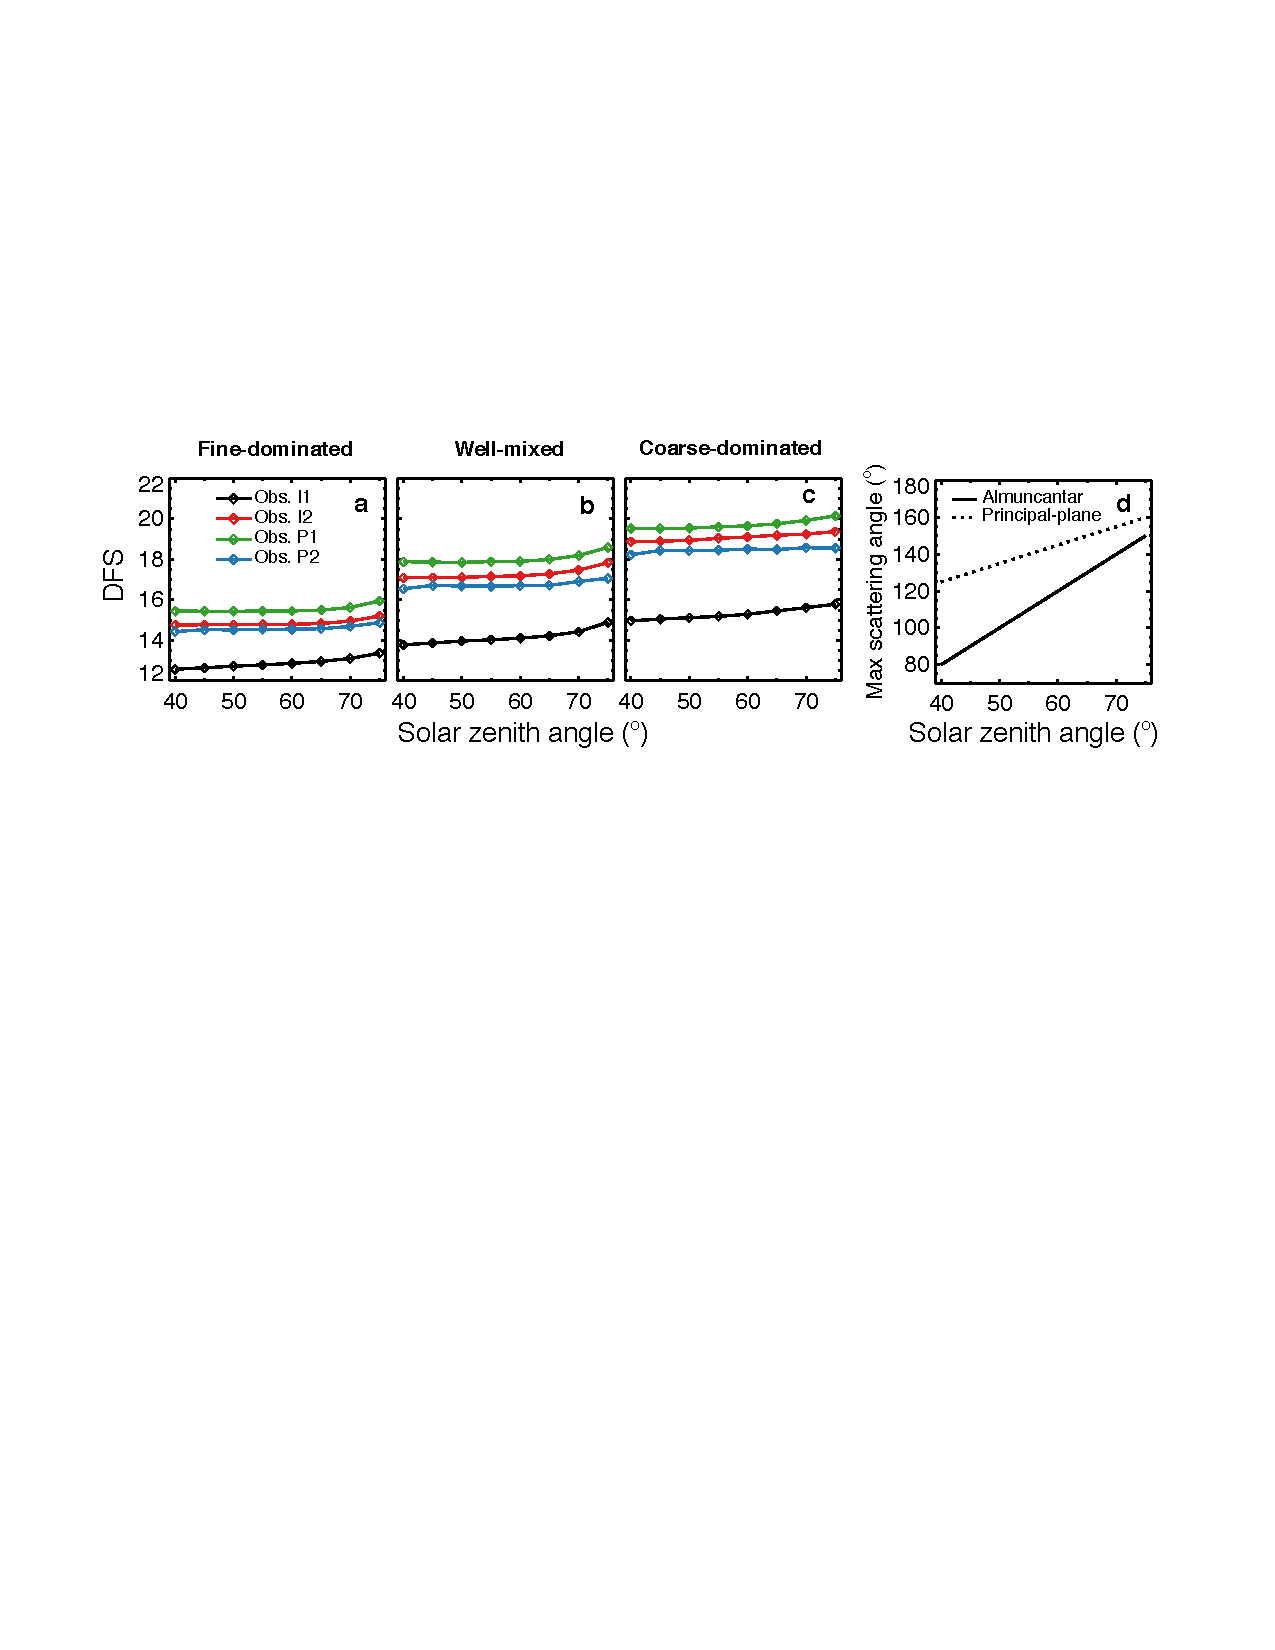
\includegraphics[width={\textwidth}]{figures/info05.pdf}
  \caption{Degree of freedom for signal (DFS) as a function of solar zenith
angle for retrieving all 22 parameters when using aerosol type of (a)
fine-dominated,  (b) well-mixed, and (c) coarse-dominated. Four differently
colored-curves denote four observation scenarios defined in Table 1. Panel (d)
shows the maximum scattering angles that can be reached by the almucantar and
the principal-plane scans.}
  \label{fig:infodfs1}
\end{figure}

We illustrate the DFS components $\Abf_{i,i}$ in Figure \ref{fig:infodfspsd1} 
for the $V_0$, $\reff$ and $\veff$, and in Figure \ref{fig:infodfsmr} and
\ref{fig:infodfsmi} for the $\mreal$ and $\mimag$, respectively. Also shown
in those figures are the a posteriori errors, which are the diagonal elements
of $\hat{\Sbf}^{\frac{1}{2}}$. It should be noted that errors for $V_0$,
$\reff$, and $\veff$ are in terms of relative uncertainties (\%), while errors
in the $\mreal$ and $\mimag$ are absolute quantities. Curves of four different
colors in each panel indicate these defined four observation scenarios and
are averages for the three aerosol types. Error bars represent one fifth of 
the standard deviations among the three aerosol types (the use of the o
ne-fifth scale is only for plotting purpose). These error bars thus depict
the variability of the DFS component and retrieval error over the fine-mode 
fraction ($\fmfv$). Mean retrieval uncertainties averaged over various solar 
zenith angles are summarized in Table \ref{tab:infoerr}. We discuss these results 
for each retrieved parameter in detail as following. 

\subsubsection{Aerosol PSD}

Among the 22 elements in the state vector, the $V_0$, $\reff$ and $\veff$ 
describe the aerosol PSD. According to Figure \ref{fig:infodfspsd1}a-c, 
observations in the scenario P1 (green curves) always yield the highest 
DFS components for inferring PSD parameters in both the fine and coarse modes,
followed by observations from the scenarios I2 (red) and P2 (blue), and lastly
the scenario I1 (black). As a consequence, the \textit{a posterior} errors are
found smallest for the scenario P1 and largest for the scenario I1 (Figure 
\ref{fig:infodfspsd1}d-e). Retrieval errors in the scenario I1 (black curves)
are 5--15\% for $V_0$, 5--9\% for $\reff$, and 20--30\% for $\veff$,
which vary with solar zenith angles. In contrast, retrieval errors in the
scenario P1 (green curves) are reduced to $\sim$2.5\%(3\%), 1\%(3.5\%), and 
7\%(20\%) for the fine (coarse) mode. From observations in the scenarios P2
and I2, one can retrieve $V_0$, $\reff$, and $\veff$ of errors lying between
the scenarios I1 and P1, though slightly larger in the scenario P2. 
In addition, higher DFS components and smaller retrieval errors are found for
the fine-mode parameters than those for the coarse mode, because radiances
and polarization are in particular more sensitive to aerosol parameters in the
fine mode as shown in the contrast between the Figures \ref{fig:infoenjf} and 
\ref{fig:infoenjc}

%% Figure DFS and error of PSD 
\begin{figure}[t]
  \centering
  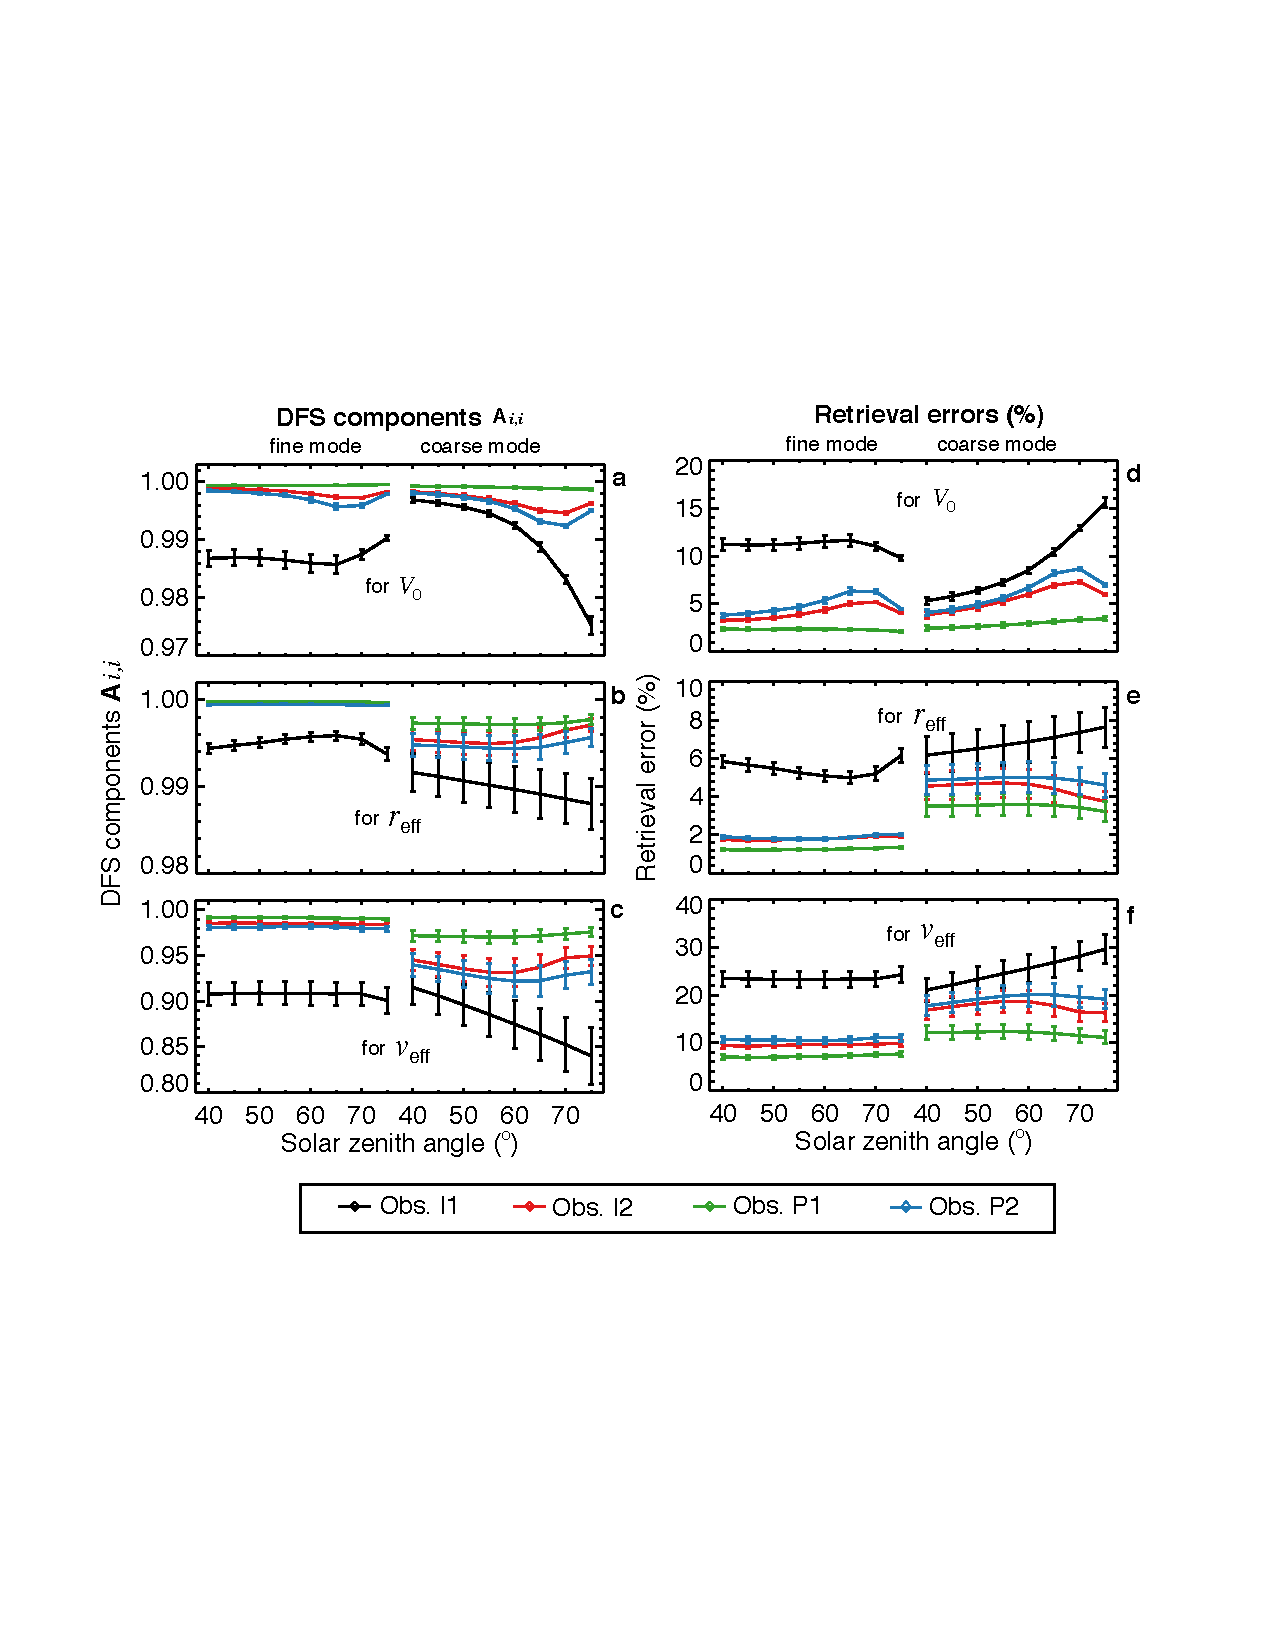
\includegraphics[width={\textwidth}]{figures/info06.pdf}
  \caption{DFS components (left column) and retrieval uncertainty (right
column) as a function solar zenith angle with different observation scenarios
defined in Table \ref{tab:infoy}. Quantities are averages for three aerosol 
types defined in Table \ref{tab:infoopt}, and error bars represent 
one fifth of standard deviation. Three rows from top to bottom are 
respectively for retrieving $V_0$, $\reff$, and $\veff$. In
each panel, shown in the left is for the fine mode and in the right is for the
coarse mode.}
  \label{fig:infodfspsd1}
\end{figure}

We also note that, in the scenario I1, DFS components for the coarse-mode
parameters decrease with increasing solar zenith angle, while no obvious trend
can be found for the fine-mode parameters. This can be explained by the low
sensitivity of the $\ialm$ to the coarse-mode $V_0$, $\reff$, and $\veff$ at
large scattering angles as showed in Figure \ref{fig:infoenjc}a-c. Higher 
sensitivities occur at scattering angles below $\sim$30$^\circ$; the increase
in SZA results in a smaller number of measurements in the near-forward 
scattering angular regions, and thus leads to larger retrieval errors. 
However, these trends turn to be weaker or negligible in other observation 
scenarios, especially the scenario P1. We can understand this from two aspects.
First, observations from principal plane can add additional measurements near
the forward scattering region. Second and most importantly, the added 
polarization measurements in the scenarios P1 and P2 contain additional 
information that is independent of the scattering angle limitation as 
discussed in the section \ref{subsec:enj}.

Overall, the increase in DFS components by adding polarization measurements is
less than 0.1 for retrieving $V_0$, $\reff$, and $\veff$, because radiances alone
contain abundant information. The retrieval accuracy in aerosol PSD from
observations of all scenarios exceeds the requirements for better quantifying
aerosol climate radiative forcing identified by \citet{Mishchenko04}. Even
so, the addition of multi-band $\dolppp$ measurements to the inversion can
still yield up to $\sim$70\% retrieval error reduction in the fine-mode and up
to $\sim$50\% reduction in the coarse-mode aerosol PSD parameters. 

\subsubsection{Refractive indices}

As shown in Figure \ref{fig:infodfsmr}a-b, different magnitudes prevail in
the DFS components for the $\mreal$ between fine and coarse modes and among
different observation scenarios. For example, DFS components for aerosols in
the fine mode overreach 0.8 at all four wavelengths in the scenario I1; while
the counterparts in the coarse mode approach 0.5 at 1020 nm and are less than
0.2 for the other three wavelengths. This is due to the weaker sensitivity of
almucantar radiances to the coarse-mode $\mreal$  (as in Figure
\ref{fig:infoenjc}d) comparing to that for aerosol in the fine
mode (as in Figure \ref{fig:infoenjf}d). In general, adding the $\dolpalm$,
$\ipp$, or both the $\ipp$ and $\dolppp$ in the inversion increases the DFS
components for $\mreal$ of aerosols in both the fine and the coarse modes. 
Particularly, DFS components achieve the most significant rise in the scenario
P1 by climbing to 0.95--1.0 in the fine mode and to 0.4--0.8 in the coarse 
mode. Also shown in Figure \ref{fig:infodfsmr}a, an increasing pattern with
solar zenith angles is found in the DFS components for the fine-mode aerosol
at larger wavelengths because stronger sensitivity occurs in larger scattering
angles.

%% Figure DFS and error of mr
\begin{figure}[p]
  \centering
  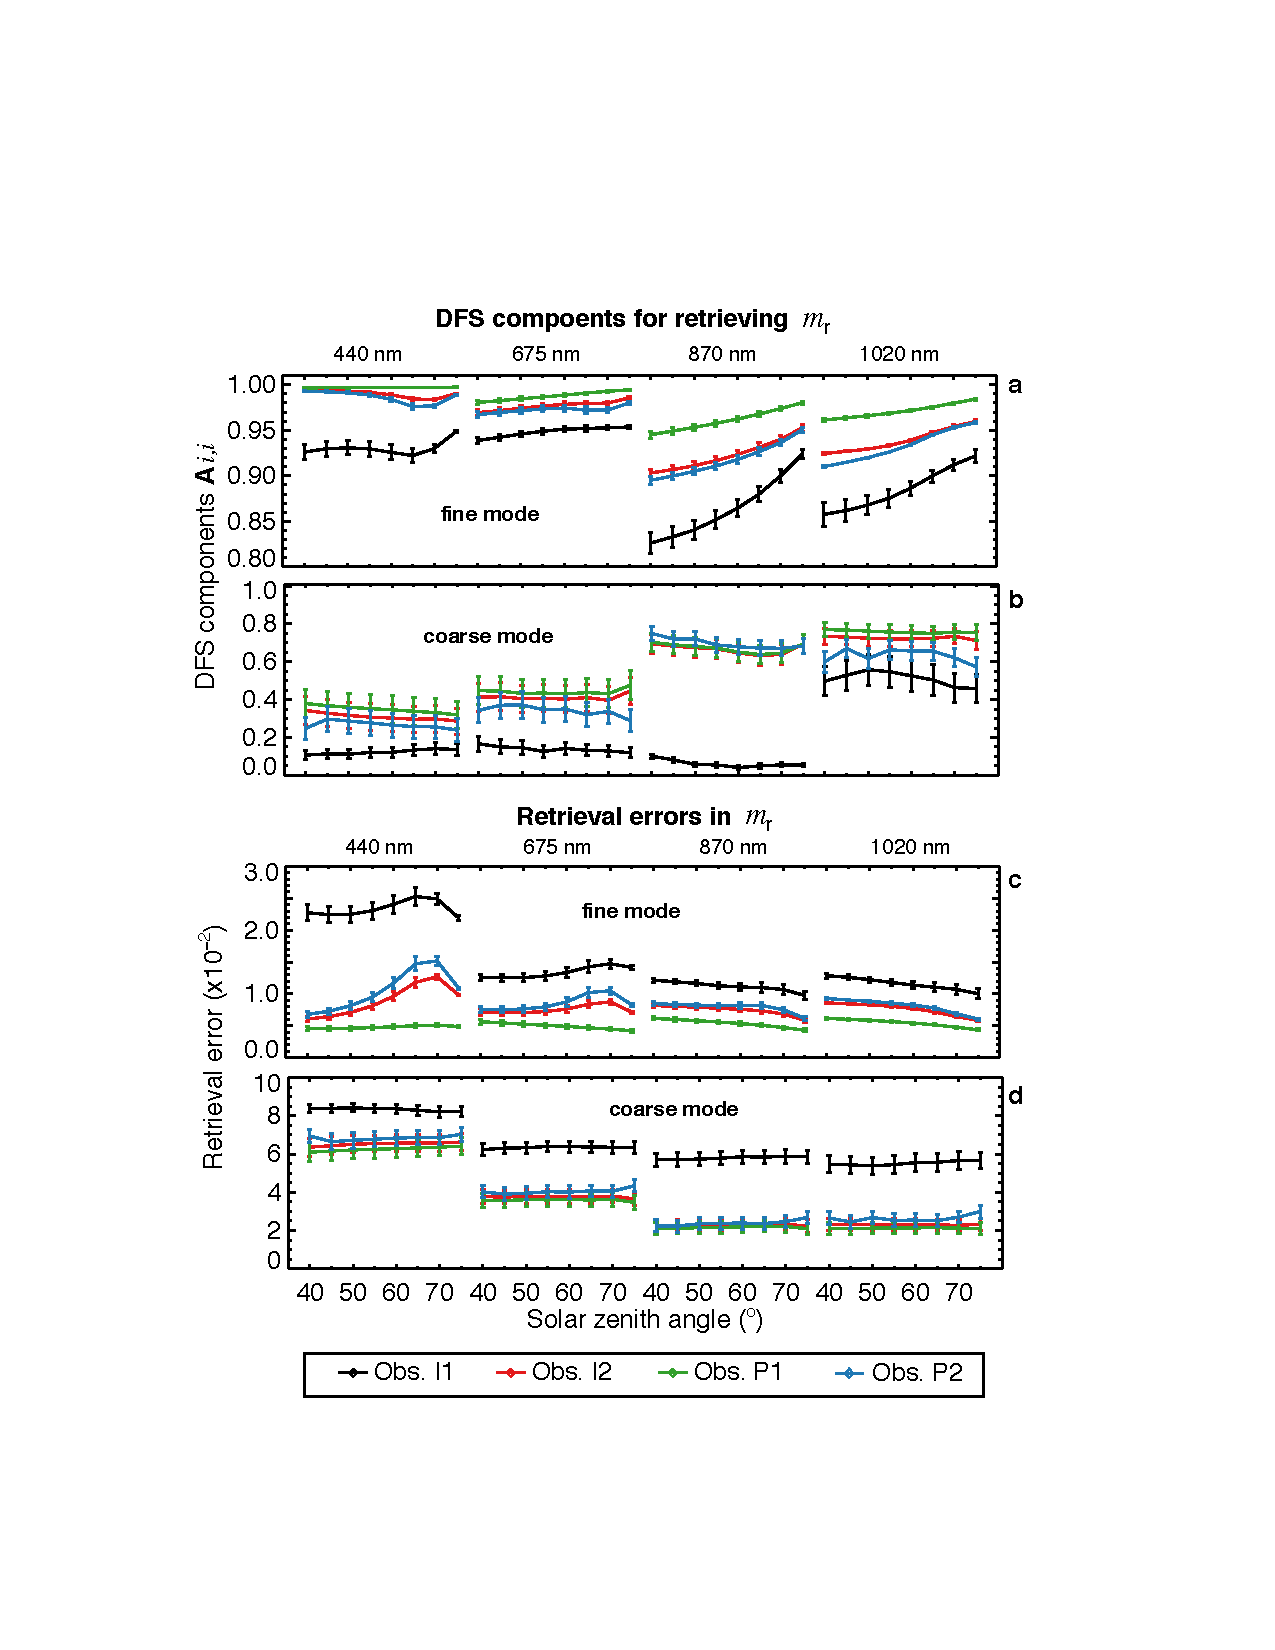
\includegraphics[width={0.9\textwidth}]{figures/info07.pdf}
  \caption{Same as Figure \ref{fig:infodfspsd1} but for DFS components (a-b) and 
retrieval uncertainty (c-d) for retrieving real part refractive index $mreal$ 
in four wavelength bands. (a) and (c) are for the fine aerosol mode, while 
(b) and (d) for the coarse mode. }
  \label{fig:infodfsmr}
\end{figure}

%% Figure DFS and error of mi
\begin{figure}[p]
  \centering
  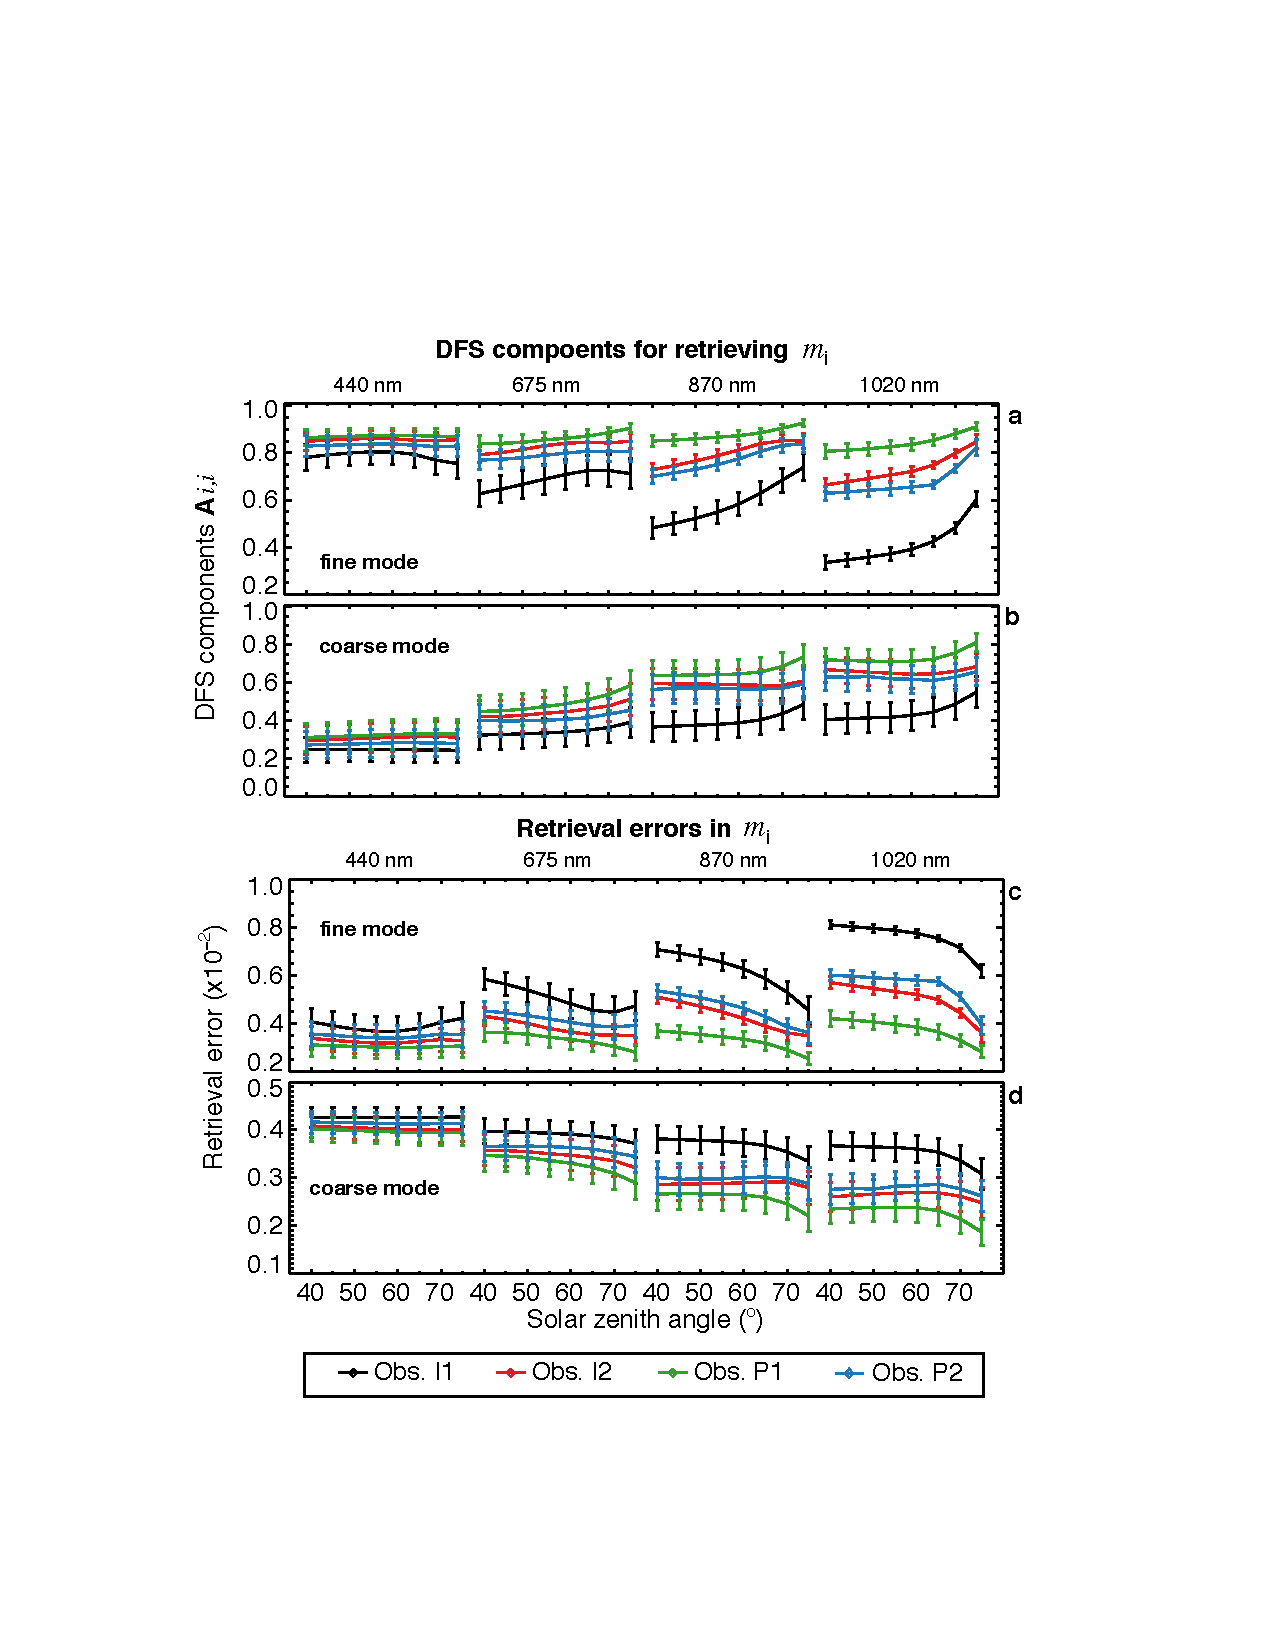
\includegraphics[width={0.9\textwidth}]{figures/info08.pdf}
  \caption{Same as Figure \ref{fig:infodfsmr} but for retrieving imaginary 
part refractive index $\mimag$.}
  \label{fig:infodfsmi}
\end{figure}

As expected, the retrieval of $\mreal$ can be more accurate by adding additional
measurements. According to Figure \ref{fig:infodfsmr}c-d, the \textit{a
posteriori} error in $\mreal$ averaged on the four spectral bands is 
$\sim$0.015 (0.065) for aerosols in the fine (coarse) mode from measurements
in the scenario I1. In contrast, it is reduced to 0.008 (0.037), 0.005 (0.035), 
and 0.009 (0.040) in the scenarios I2, P1, and P2, respectively. 
Retrieval errors in the coarse-mode $\mreal$ are larger in shorter
spectral wavelengths because of weaker sensitivity to the $\ialm$ and DOLP. 
For instance of the scenario P1, it is about 0.06 at 440 nm, 0.035 at 675 nm, 
and 0.02 at 870 and 1020 nm. 

The DFS components for the $\mimag$ are shown in Figure \ref{fig:infodfsmi}a–b,
and the corresponding retrieval errors in $\mimag$ are displayed in 
Figure \ref{fig:infodfsmi}c–d. Similar to those for the $\mimag$, DFS
components for retrieving the $\mimag$ are larger in the fine mode and show
an increasing pattern with the solar zenith angle. Observations in the scenario
P1 always yield largest DFS components and smallest retrieval error for the
$\mimag$, followed by the scenarios P2 and I2. Observations in the scenario I1
offer the $\mimag$ retrieval with largest error. If averaged on the solar
zenith angles and aerosol types, the retrieval error in the $\mimag$ is 
0.006 (0.004) for aerosol in the fine (coarse) mode in the scenario I1, and 
can be reduced to 0.003 (0.003) in the scenario P1. 

%% Table of retrieval error 
\begin{table}[t]
  \centering
  \small
  \caption{Error for retrieved and derived parameters among \textit{a priori},
          \textit{a posteriori}, and Glory characterization\textsuperscript{a}.}
  \label{tab:infoerr}
  \begin{tabular}{p{4em} C{4em} C{4em} C{4em} C{5em} C{5em} C{5em} }
  \toprule
  & \multicolumn{5}{c}{Error in retrieved parameters} \\
  \cmidrule(r){2-6} 
  Entries & $V_0$ (\%)& $\reff$ (\%)& $\veff$ (\%)& $\mreal$ & $\mimag$ & $\assa$ \\
  \midrule
   A priori & 100/100 & 80/80 & 80/80& .15/.15 & .01/.05 & - \\
   Obs. I1 & 11./9.0 & 5.5/6.8 & 23/25 & .015/.065 & .0057/.0038 & .037/.085 \\
   Obs. I2 & 4.1/5.5 & 1.8/4.4 & 10/18 & .008/.037 & .0041/.0032 & .024/.073 \\
   Obs. P1 & 2.3/2.9 & 1.3/3.5 &7.2/12 & .005/.035 & .0033/.0030 & .019/.068 \\
   Obs. P2 & 4.9/6.2 & 1.9/4.9 & 11/19 & .009/.040 & .0044/.0034 & .026/.076 \\
   Glory$^b$ & –     & 10 & 40 & .02  & – & .03 \\
  \bottomrule
  \multicolumn{7}{m{35em}}{\textsuperscript{a}Results of our work are averaged
values for three aerosol types and for solar zenith angles from 
40$^\circ$ to 70$^\circ$. \newline \textsuperscript{b}Referred to
\citet{Mishchenko04}.}  
  \end{tabular}
\end{table}

\subsubsection{Single scattering albedo}

Note that the aerosol single scattering albedo $\assa$ is an intermediate rather
than a directly retrieved parameter. The error in $\assa$ can be estimated
from the $\hat{\Sbf}$ with the equation \eqref{eq:zeta}. The $\assa$ for each
aerosol mode uniquely depends on the light wavelength and aerosol 
microphysical parameters including $\reff$, $\veff$, and $\mreal$ and $\mimag$,
although the $\mimag$ impacts $\assa$ most significantly \citep{Hansen74}.
Required derivatives of $\assa$ to these parameters in the equation
\eqref{eq:zeta} can be obtained from the linearized Mie code (section
\ref{subsec:mie}) integrated into the UNL-VRTM. We calculated uncertainties 
in the $\assa$ for each wavelength and each aerosol type, and the averaged 
values are summarized in Table \ref{tab:infoerr}. Observations in these four 
scenarios can  retrieve $\assa$ with the uncertainty of 0.037, 0.024, 0.019, 
and 0.026 for  the fine mode, and 0.085, 0.073, 0.068, and 0.076 for the coarse
mode, respectively. Thus, only the fine-mode $\assa$ retrieval with polarization
involved can meet the accuracy requirements (0.03) for accurate climate forcing
estimates \citep{Mishchenko04}. We noted that the mean uncertainty in the
coarse-mode $\assa$ exceeds 0.06 in all of these four scenarios, but higher
accuracy may be achieved under coarse-dominated conditions as shown in the
following section.  

\section{Sensitivity of Retrieval Error to AOD and $\fmfv$} 
\label{sec:infosensi}

The performance of retrieval usually varies with aerosol conditions like
the aerosol loading and the prevalence of aerosol in either the fine or
the coarse modes (e.g., fine-mode volume fraction, $\fmfv$). As a result,
uncertainties in aerosol retrievals can depend much more strongly on the
AOD than they do on the properties of an individual aerosol model
\citep{Knobelspiesse12}. For the same reason, the inversion of
refractive indices and $\assa$ in the current AERONET algorithm is confined
to the condition when the 440-nm AOD is larger than 0.4
\citep{Dubovik00b, Holben06}. Our above analysis, which focused on three
aerosol types by a constant AOD value at 440 nm (${\taua}_{440}$=1.0), is
insufficient to represent variable global conditions. At the same time,
we also found noticeable variability of the DFS components and a
posteriori errors existing among three aerosol types with different
$\fmfv$, especially for the coarse-mode parameters. Thus, it is necessary
to investigate how aerosol conditions affect the retrieval error, in
order to answer the question: under what aerosol conditions the AERONET
measurements (with and without polarization) are capable to yield
retrievals with satisfied accuracy?

%% Figure DFS in sensitivity
\begin{figure}[t]
  \centering
  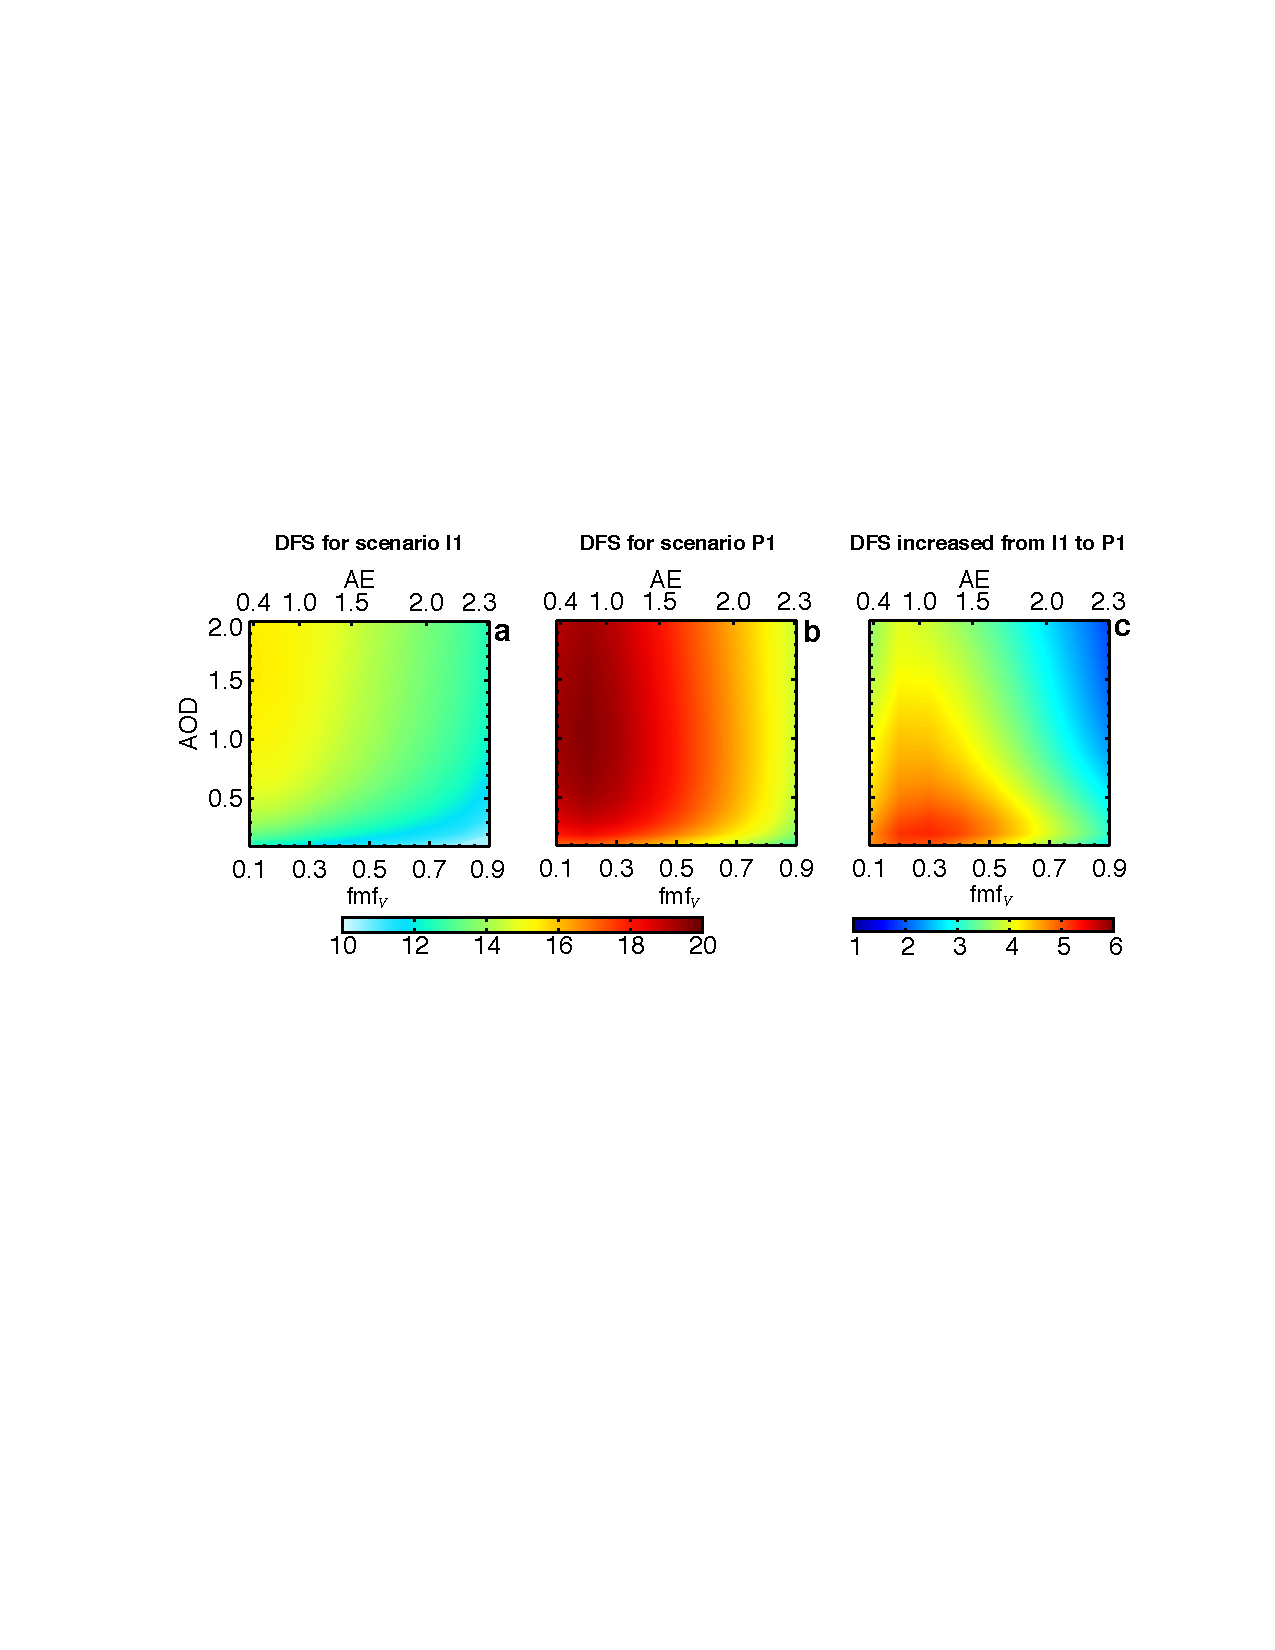
\includegraphics[width={\textwidth}]{figures/info09.pdf}
  \caption{Contours of DFS as a function of $\fmfv$ and AOD in scenarios
I1 (a) and P1 (b). (c) the difference of DFS between (a) and (b).
Simulations are for solar zenith angle of 55$^\circ$. The top abscissa denotes
Ångström exponent (AE).}
  \label{fig:infodfs2}
\end{figure}

We expand our analysis for the ${\taua}_{440}$ ranging from 0.1 to 2.0 
and for the $\fmfv$ from 0.1 to 0.9. In practice, the $\fmfv$ is 
inaccessible prior to inversion. Instead, we use the 
Ångström exponent (AE) from 870 to 1020 nm together with
${\taua}_{440}$ to define the aerosol conditions, because the AE
in the longer paired wavelength is highly related to the $\fmfv$
\citep{Schuster06} and immediately available from the AERONET direct sun 
measurements. With the aerosol properties defined in the Table
\ref{tab:infoy},the $\fmfv$ from 0.1 to 0.9 gives AE values from
0.35 to 2.3. We exclude the scenarios of I2 and P2 in our following
analysis, because the scenario P1 demonstrates the most superior
performance and is also the focus of our algorithm development.

%% Figure error fine-mode in sensitivity
\begin{figure}[pt]
  \centering
  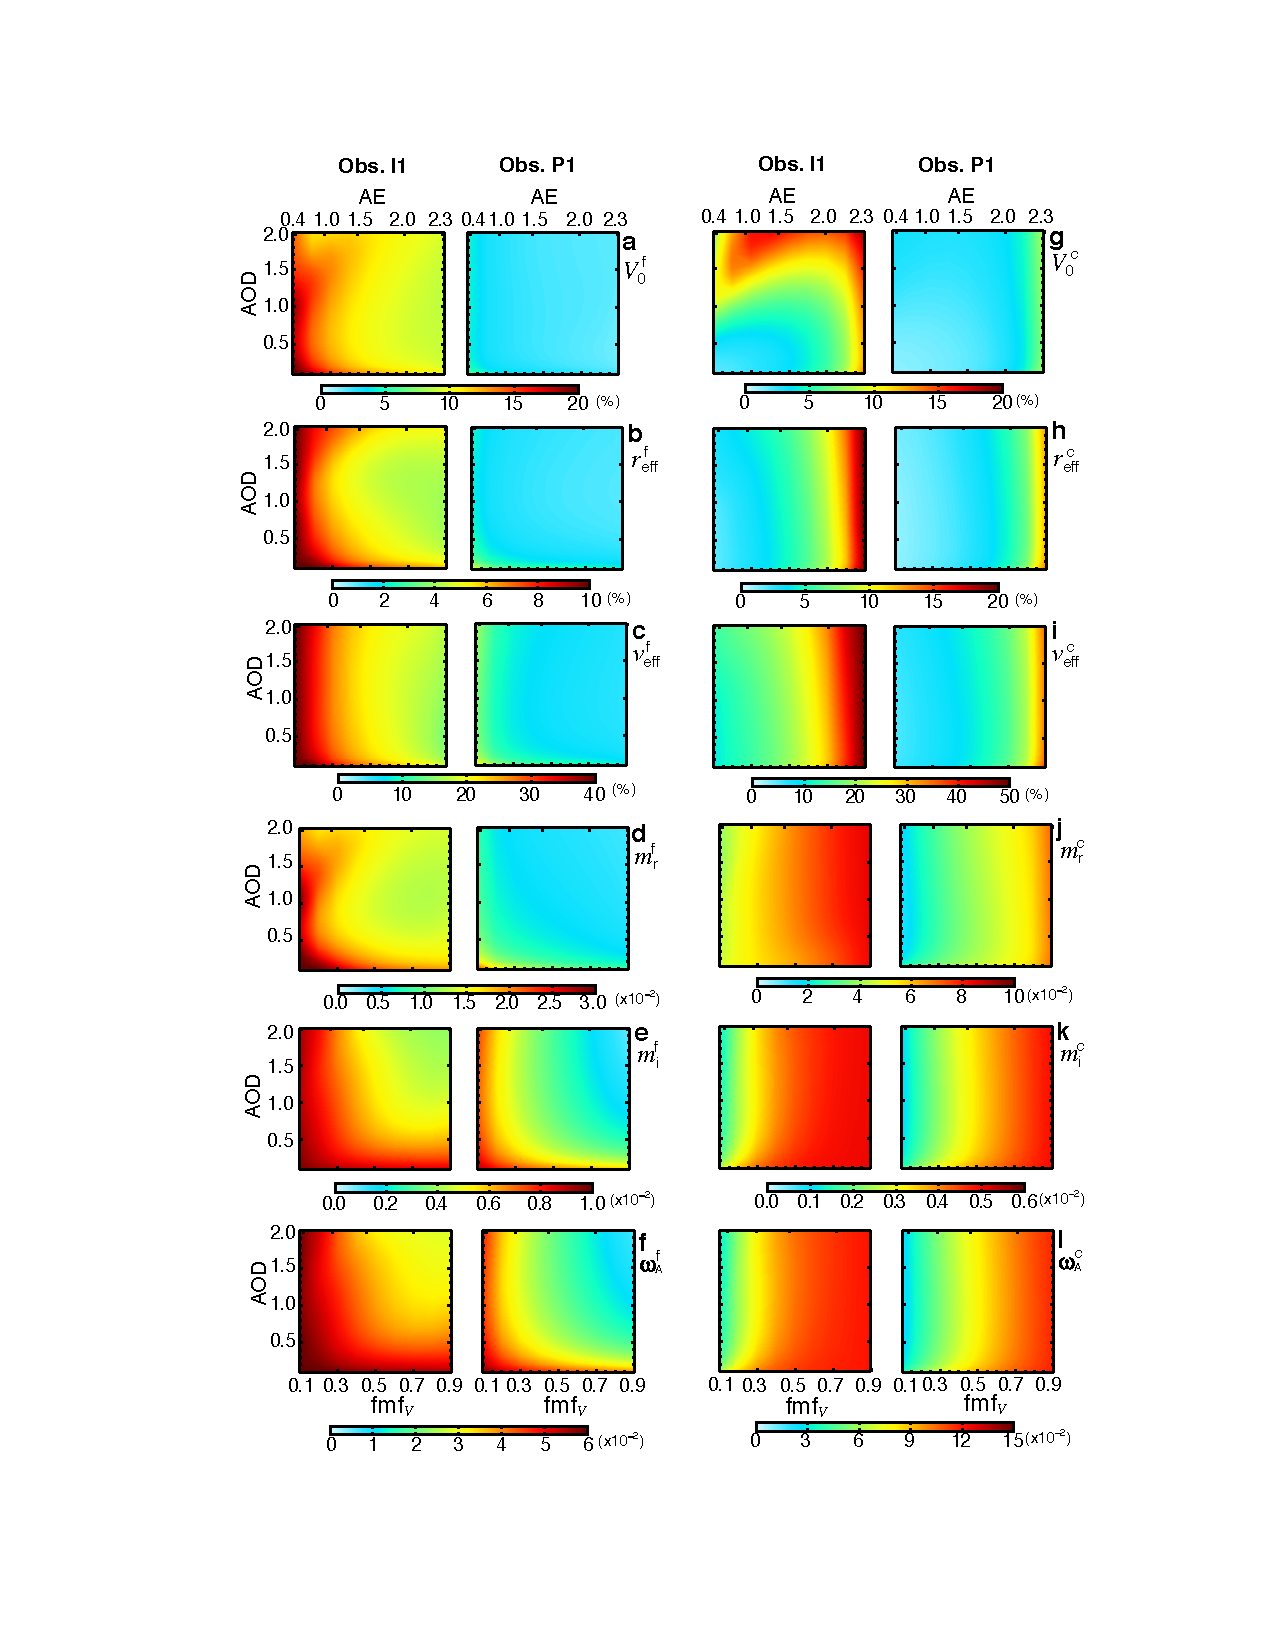
\includegraphics[width={\textwidth}]{figures/info10.pdf}
  \caption{Retrieval uncertainties as a function of $\fmfv$ (or AE) and
AOD for each individual aerosol parameters in the \textit{fine} mode: (a) $V_0$,
(b) $\reff$, (c) $\veff$, (d) $\mreal$, (e) $\mimag$, and (f) $\assa$.
Two sub-panels in each panel indicate observations in the scenarios 
I1 and P1, respectively. Simulations are for solar zenith angle of
55$^\circ$. The x- and y-axis are identical to those in Figure
\ref{fig:infodfs2}. Relative uncertainties are shown for
$V_0$, $\reff$ and $\veff$, while absolute errors for $\mreal$, $\mimag$, 
and $\assa$. Retrieval errors for $\mreal$, $\mimag$, 
and $\assa$ are averaged values over the four spectral bands.}
  \label{fig:infoerrf}
\end{figure}

%% Figure error coarse-mode in sensitivity
\begin{figure}[pt]
  \centering
  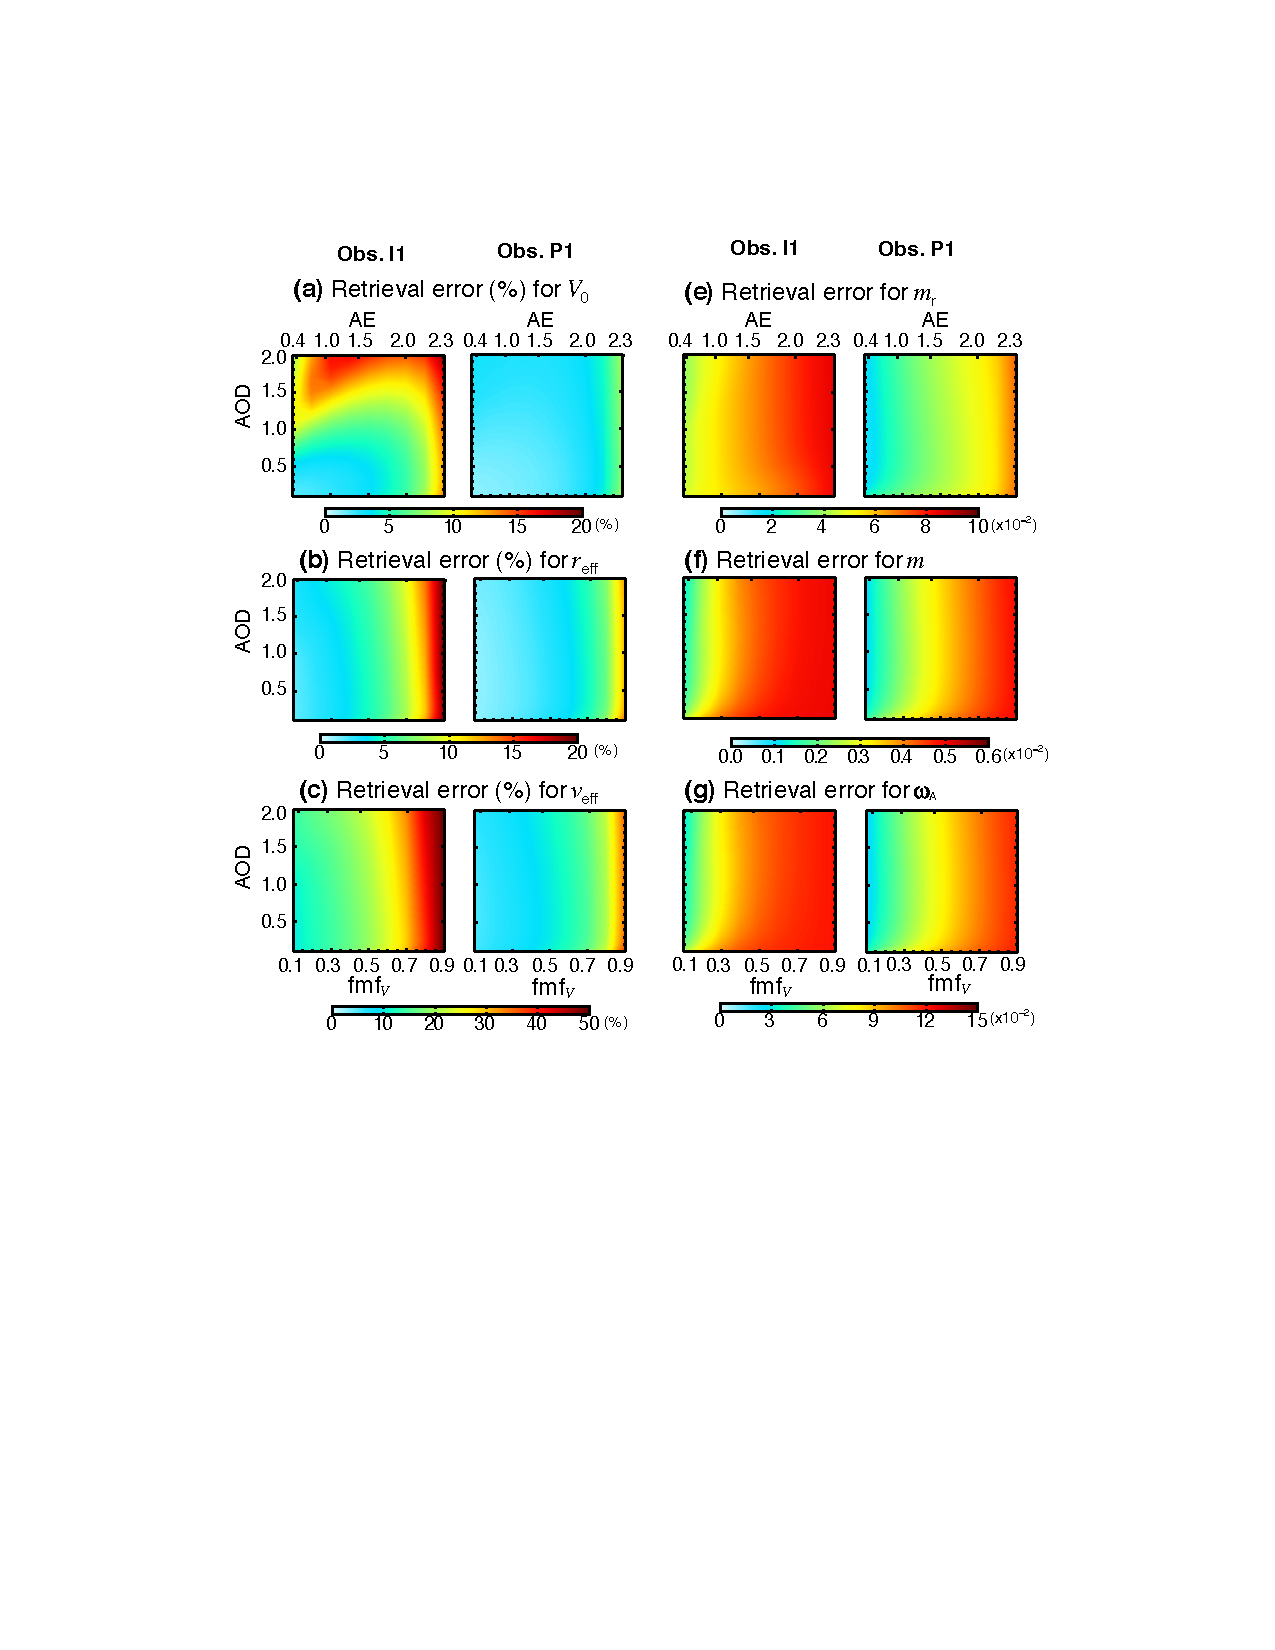
\includegraphics[width={\textwidth}]{figures/info11.pdf}
  \caption{Same as Figure \ref{fig:infoerrf}, but for aerosol parameters in 
the \textit{coarse} mode.}
  \label{fig:infoerrc}
\end{figure}

Figure \ref{fig:infodfs2}a--b display the contours of DFS as a function 
of the AE (or $\fmfv$) and ${\taua}_{440}$ in the scenarios I1 and P1, 
respectively. We found that the DFS decreases with an increasing AE and
$\fmfv$ for the same AOD. This is attributed to the fact that the 
coarse-mode parameters are more difficult to retrieve than their 
fine-mode counterparts, restrained by their weaker sensitivities to 
the $\ialm$ and the $\dolppp$. Thus, the decrease in the coarse-mode 
fraction significantly reduces the aerosol information for coarse-mode 
parameters but retain the information for fine-mode parameters, resulting in 
decreases in the total DFS. We also notice from Figure
\ref{fig:infodfs2}a that the DFS increases with an increasing AOD in the
scenario I1. However, AOD change has less impact in the scenario P1
(Figure \ref{fig:infodfs2}b). For example, the DFS values are lower than 14 
when AOD < 0.4 in the scenario I1, whereas even larger DFS can be found in 
the scenario P1 when AOD $<$ 0.2. Therefore, we may expect that the inversion 
in the scenario P1 will be capable to retrieve aerosol parameters in conditions
of lower aerosol loading, and may bring down the ${\taua}_{440}$ threshold of 
0.4 from the current AERONET inversion algorithm to retrieve the refractive
index and $\assa$. Finally, as indicated in Figure \ref{fig:infodfs2}c, 
the addition of $\ipp$ and $\dolppp$ in the inversion can add 2--5 pieces of 
useful information. Such improvement occurs in all aerosol conditions but is 
more dominated when enough coarse particles are present: $\fmfv<0.5$ (or
AE$<1.6$), in which the radiance-only inversion usually yields a large 
retrieval error for the fine-mode aerosol. 

In Figures \ref{fig:infoerrf} and \ref{fig:infoerrc}, we show the contours of
the a posteriori error $\hat\epsilon$ in the scenarios I1 and P1 for the 
individual fine-mode and coarse-mode parameters, respectively. Overall, 
observations in scenarios P1 offer more accurate retrievals for all parameters
in both the fine and the coarse aerosol modes. In both scenarios, the
$\hat\epsilon$ decreases for fine-mode parameters and increases for 
coarse-mode parameters with increasing the AE (or $\fmfv$) for same
${\taua}_{440}$, indicating that the relative contribution
of fine and coarse modes determines the relative information of each
mode. Extreme cases are $\fmfv$ of 1 or 0, i.e., the absence of the
coarse- or fine-mode aerosols, which certainly will only allow a
mono-modal retrieval. Thus, the bi-modal retrieval, especially for
refractive indices, requires that aerosols reach certain mixture
conditions to contain enough information for both modes. For example in
the scenario I1, while the fine-mode $\reff$ can be well retrieved with 5\%
accuracy when the $\fmfv>0.2$ at ${\taua}_{440}$ of 0.5 (Figure
\ref{fig:infoerrf}b), the $\fmfv>0.3$ is required to ensure the
$\hat\epsilon<0.02$ in the fine-mode $\mreal$ (Figures
\ref{fig:infoerrf}e). Comparing to the change of the $\fmfv$, the change of
${\taua}_{440}$ has less impact on the $\hat\epsilon$ of the PSD parameters;
and this impact occurs in low aerosol loadings. For example, Figure
\ref{fig:infoerrf}g shows that a minimum of $\sim$0.4
for ${\taua}_{440}$ is required in the scenario I1 to guarantee a retrieval
error in the fine-mode $\assa$ less than 0.04 when $\fmfv=0.5$. 

%% Table of retrieval error 
\begin{table}[t]
  \centering
  \small
  \caption{Required aerosol conditions (${\taua}_{440}$ and AE) to achieve
anticipated retrieval accuracy $<\epsilon>$ for observations in scenario 
I1 and P1.}
  \label{tab:infosensi}
  \begin{tabular}{p{3em} R{3em} R{6em} R{6em} R{6em} R{6em} }
  \toprule
  & & \multicolumn{2}{c}{Scenario I1} & 
      \multicolumn{2}{c}{Scenario P1}\\
  \cmidrule(r){3-6}
  $\xbf$ &  $<\epsilon>$ & ${\taua}_{440}$ & AE &  ${\taua}_{440}$ & AE \\
  \midrule
  $V_0\fine$     & 10\% & >0.3 & >1.5 & \textsuperscript{a}All & All \\ 
  $V_0\coarse$   & 10\% & <1.3 & <2.2 & All & All \\
  $\reff\fine$   & 5\%  & >0.3 & >1.3 & All & All \\
  $\reff\coarse$ & 10\% & All  & <2.0 & All & <2.2 \\
  $\veff\fine$   & 20\% & >0.3 & >1.5 & All & All \\
  $\veff\coarse$ & 30\% & All  & <1.8 & All & <2.2 \\
  $\mreal\fine$  & 0.02 & >0.4 & \textsuperscript{b}\textbf{>1.0} & All & All \\
  $\mreal\coarse$& 0.04 & All  & \textbf{<1.0} & All  & <1.8 \\
  $\assa\fine$   & 0.04 & >0.6 & \textbf{>1.5} & >0.2 & >0.7 \\
  $\assa\coarse$ & 0.08 & >0.2 & \textbf{<1.1} & All  & <1.6 \\
  \bottomrule
  \multicolumn{6}{p{35em}}{
   {\textsuperscript{a}}‘All’ indicates conditions:
$0.1<{\taua}_{440}<2.0$ and $0.35<\text{AE}<2.3$; \newline
   {\textsuperscript{b}}2Underlined bold indicate conditions that cannot
allow bi-modal retrievals.}
  \end{tabular}
\end{table}

From the Figures \ref{fig:infoerrf} and \ref{fig:infoerrc}, we can identify 
required aerosol conditions in terms of the AE and ${\taua}_{440}$ in order
to achieve certain anticipated accuracy $<\epsilon>$, which are summarized
in Table \ref{tab:infosensi}. Clearly, observations with polarization can enable 
retrievals of same accuracy in a lower aerosol loading. For example, the 
retrieval accuracy of 10\% for the $V_0$ and $\reff$ and 30\% for the
$\veff$ in the fine mode requires ${\taua}_{440}$ to be larger than 0.3 for 
inversion in the scenario I1 (Figure \ref{fig:infoerrf}a--c). In
contrast, inversion in the scenario P1 can easily ensure retrievals of
the same accuracy when ${\taua}_{440}$ is 0.1. For the fine-mode
$\mreal$ retrieval, an accuracy of 0.04 requires ${\taua}_{440}>0.4$ for the
inversion I1 but ${\taua}_{440}>0.2$ for the inversion P1 (Figure
\ref{fig:infoerrf}e). Moreover, the radiance-only inversion
is unable to resolve the bi-modal $\mreal$ and $\assa$ under any circumstance,
because AE$>$1.5 is necessary for retrieving the fine-mode $\assa$
(Figure \ref{fig:infoerrf}g), meanwhile AE$<$1.1 is required for its 
coarse-mode retrieval (Figure \ref{fig:infoerrc}g). This agrees with 
\citet{Dubovik00b} in that the retrieval of refractive indices for both fine
and coarse mode is essentially non-unique due to limited information in the
AERONET (radiance-only) observations. In contrast, observations in the
scenario P1 can allow bi-modal retrievals of the $\mimag$ and $\assa$ when 
$0.7<\text{AE}<1.6$ and ${\taua}_{440}>0.2$ (Figures \ref{fig:infoerrf}g
and \ref{fig:infoerrc}g). Therefore, our retrieval algorithm is designed
to use observations of scenario P1 to retrieve bi-modal refractive indices 
when ${\taua}_{440}$ and AE reach these criteria. In aerosol conditions beyond
the criteria, bi-modal PSD along with a mono-modal refractive index will be 
retrieved by assuming the refractive index is independent of the aerosol mode.

\section{Summary} \label{sec:infosummary}

In an effort to improve the AERONET inversion by including additional
polarization measurements, this study examines the potential
microphysical aerosol information contained in the AERONET
photo-polarimetric observations. We have focused our analysis on how the
added polarization measurements impact on the retrieval accuracy the in
aerosol particle size distribution (PSD), spectral refractive index, and
single scattering albedo $\assa$. A numerical testbed has been constructed
to generate the synthetic AERONET radiance and degree of linear
polarization (DOLP) over 440, 675, 870, and 1020 nm. We considered four
scenarios of observations to whether or not include the DOLP for the
inversion, i.e., (I1) direct Sun AOD and almucantar sky radiances, (I2)
observations in the scenario I1 with additional radiance measurements in
the solar principal plane, (P1) observations in the scenario I2 plus
polarization measurements in the solar principal plane, and (P2)
observations in the scenario I1 plus almucantar polarization.
Measurements in the scenario I1 are those used in current AERONET
inversion algorithm, and thus represent a control experiment. For each
observation scenario, we also considered three aerosol types to
represent general aerosol climatology.  The Bayesian statistical
approach then was applied to relate information contained in those
synthetic data and retrieval errors in aerosol physical parameters to
the instrumental as well as the a priori characteristics. Then the
error-normalized Jacobian, degree of freedom for signal (DFS), and the a
posteriori error in each individual retrieved parameter were presented
as function of solar zenith angle for these observation scenarios. 

The results show a remarkable increase in information by adding
additional polarization and/or radiances into the inversion. Overall,
observations in the scenario P1 yield the highest DFS, which is larger
than that in the scenario I1 by 2--5 for all defined aerosol types. This
can be understood that polarization measurements in the solar principal
plane, in comparing with sky radiances in solar almucantar, have
complementary sensitivities with respect to retrieved aerosol
parameters. Also, measurements in the principal plane allow a wider
range of scattering angles and supplies more information on aerosol
backscattering. In scenario P2, adding polarization in the solar
almucantar offer an increase of $\sim$2 pieces of information with DFS values
slightly below those in scenarios I2. We also note that the DFS
increases with increasing solar zenith angle for all cases, resulting
from more information contained in observations of a wider range of
scattering angle.

We also analyzed the DFS components and the a posteriori uncertainty for
each individual retrieved parameter. As expected, the smallest retrieval
errors were always found in the scenario P1: 2.3\% (2.9\%) for the volume
concentration, 1.3\% (3.5\%) and 7.2\% (12\%) for the effective radius and
effective variance, 0.005 (0.035) for the real part of refractive index,
and 0.019 (0.068) for the single scattering albedo in the fine (coarse)
mode. These values represent an error reduction from the scenario I1 of
79\% (57\%), 76\% (49\%), 69\% (52\%), 66\% (46\%), and 49\% (20\%), respectively.
Uncertainties in retrieved parameters averaged among these three aerosol
types are summarized in the Table \ref{tab:infoerr} for each observation scenario. 

Seeking to answer under what conditions the inversions can achieve a
mode-resolved aerosol refractive index and $\assa$, we further investigated
how the AOD (${\taua}_{440}$) and fine/coarse modal domination (in terms of
Ångström exponent, or AE) influence the retrieving accuracy from
observations in the scenarios I1 and P1. We found that adding
principal-plane polarization measurements can increase the DFS by up to
$\sim$5 in cases dominated by coarse-mode particles ($\fmfv<0.5$), in which
the radiance-only inversion usually yields larger retrieval uncertainty
for fine-mode aerosol. As a consequence, these photo-polarimetric
observations can enable accurate retrievals in a lower aerosol loading
when the ${\taua}_{440}$ is 0.1, except for the fine-mode $\mreal$ retrieval that
requires ${\taua}_{440}>0.2$. The analysis also indicate that the radiance-only
inversion is unable to resolve bi-modal $\mimag$ and $\assa$ under any
circumstance. However, observations in the scenario P1 can allow
bi-modal retrievals of $\mimag$ and $\assa$ when $0.7<\text{AE}<1.6$. 
Such criteria can guide us in the practical retrieval algorithm to determine
whether a mono-modal or bi-modal retrieval of the aerosol refractive index and
$\assa$. In aerosol conditions beyond the criteria, bi-modal PSD along with
the mode-independent refractive index will be retrieved. 

Finally, it should be noted that in our analysis the aerosol particles
in each mode are assumed to be poly-disperse homogeneous spheres.
Although the linearized T-matrix code has been implemented in our model,
the simulation of scattering properties for large non-spherical
particles (for example spheroids) still remain computational
limitations. Our future efforts will implement non-spherical treatment
in order to more realistically represent mineral dust aerosols.

